%\documentclass[11pt,a4paper]{article}
%\documentclass[11pt,a4paper]{scrartcl}
\documentclass[11pt,a4paper,oneside]{book}
\usepackage[british,UKenglish,USenglish,english,american]{babel}
%\usepackage[a4paper, total={16cm, 23cm}]{geometry}
\usepackage[tmargin = 1.25in,bmargin = 1.25in,lmargin = 1in,rmargin = 
1in]{geometry}
\usepackage{tikz}
\usepackage{graphicx}
\usepackage{pgfplots}
\pgfplotsset{width=12cm,compat=1.9}

\usepackage{chemmacros}
\usepackage{chemfig}
%\usepackage{ghsystem}
\usechemmodule{redox}
%\usepackage{chemnum}
%\usepackage{bohr}
%\usepackage{elements}
%\usepackage{endiagram}
%\usepackage{modiagram}
%\usepackage{chemgreek}
%\usepackage{mhchem}
\usepackage{esint}
\usepackage{tabularray}

\usepackage{makeidx}
\usepackage{epstopdf}

\usepackage{amssymb}
\usepackage{mathrsfs}
%\usepackage{minted}
\usepackage{bm}
\usepackage{amsmath}
\usepackage{enumitem}
\usepackage[english]{varioref}
\usepackage[english]{babel}
\usepackage{lipsum}
\usepackage{fancyhdr}
\pagestyle{fancy} 
\usepackage{float}
\usepackage{empheq}
\usepackage[framemethod=tikz]{mdframed}
\usepackage{epstopdf}
\numberwithin{equation}{section}
\usepackage{eso-pic}
\usepackage{calc}
\usepackage{nccmath}
\usepackage{caption}
\usepackage{subcaption}
\usepackage{gensymb}
\usepackage{amsfonts,amsthm,epsfig,epstopdf,titling,url,array}
\usepackage{siunitx}
\sisetup{input-digits = 0123456789\pi}
\usepackage[symbol]{footmisc}
\usepackage{xcolor}
\usepackage{multicol}
\usepackage{boondox-cal}
\DeclareSIUnit\atm{atm}
\setcounter{secnumdepth}{3}
\setcounter{tocdepth}{3}
\usepackage{booktabs}
\usepackage{blindtext}
\usepackage{changepage}

% \usepackage{draftwatermark}
% \SetWatermarkText{DRAFT}
% \SetWatermarkScale{5}

\DeclareSIUnit\atm{atm}

\pagestyle{fancy} 
\fancypagestyle{firstpage}{
\rhead{
%	\begin{picture}(0,0) 
%			\put(-30,0){
\includegraphics[width=1cm]{figures/MCI_4C_bw.eps}} 
%	\end{picture}
}
}
\fancyhead[L]{\slshape\nouppercase{\leftmark}}
\chead{}
\rhead{
%	\begin{picture}(0,0) 
%		\put(-30,0){
\includegraphics[width=1cm]{figures/MCI_4C_bw.eps}} 
%	\end{picture}
}
\lfoot{\textit{}}
\cfoot{-\ \thepage\ -}
\rfoot{\textit{}}

\DeclareMathOperator{\rank}{rank}
\DeclareMathOperator{\atantwo}{atan2}
\DeclareMathOperator{\spn}{span}

\renewcommand{\headrulewidth}{0.4pt}
\renewcommand{\footrulewidth}{0.4pt}
\newcommand{\abs}[1]{\left|#1\right|}
\definecolor{mycolor1}{rgb}{0.97, 0.97, 0.97}
\definecolor{mycolor2}{rgb}{0.97, 0.97, 0.97}
\definecolor{tableShade}{gray}{0.9}
\newcommand{\sign}{\text{sign}}
\newcommand{\centered}[1]{\begin{tabular}{@{}l@{}} #1 \end{tabular}}
\theoremstyle{it}
\newtheorem{defn}{Definition}[chapter]
\newtheorem{assumption}{Assumption}[chapter]
\newtheorem{thm}{Theorem}[chapter]
\newtheorem{lemma}{Lemma}[chapter]
\newtheorem{corollary}{Corollary}[chapter]
\theoremstyle{definition}
%\theoremstyle{it}
\newtheorem{example}{Example}[section]

\newenvironment{myitemize_1}
{ \begin{itemize}[topsep=0pt]
		\setlength{\topsep}{2pt}		
		\setlength{\itemsep}{2pt}
		\setlength{\parskip}{2pt}
		\setlength{\parsep}{2pt}     }
	{ \end{itemize}                  }


\newmdenv[innerlinewidth=0.5pt, roundcorner=4pt,backgroundcolor=mycolor2, 
linecolor=mycolor1,innerleftmargin=6pt,
innerrightmargin=6pt,innertopmargin=6pt,innerbottommargin=6pt]{mybox}

\title{\textbf{ 
	\begin{LARGE}
		Nonlinear Observers
	\end{LARGE} \\[24pt]
	\begin{Large}
		Application to the Hydrostatic Transmissions \\[6pt] and Electrical Machinery
	\end{Large}}
}
\author{\textbf{Davide Bagnara}}

\begin{document}
	\thispagestyle{firstpage}
	\begin{mybox}
		\maketitle
		\vspace{120mm}
	\end{mybox}
	\newpage
	\tableofcontents
	\listoffigures	
	\listoftables
	\newpage
	
\chapter*{}	
\begin{adjustwidth}{50pt}{50pt}
		\textit{The present document is intended for personal use and its aim is to collect literature and case studies concerning the theme of the nonlinear systems and their control. The beginning of this document is made by a collection of applications of nonlinear control theory for hydrostatic and electrical systems. The document ends with an extended collection of appendices, where the main results of the nonlinear control theory are collected. Most of the literature, presented here, is taken from the fundamental works of H.K.~Khalil, A.~Isidori, J.~Slotine, and P.~Krause.}
\end{adjustwidth}



\chapter{Nonlinear Observer of a Hydrostatic Transmission}	
	In this chapter the design of a nonlinear observer for 
	a hydrostatic transmission is reported. At first the mathematical model of the 
	hydrostatic transmission is presented. Once the mathematical model has been outlined the 
	structure of a nonlinear observer is described as well as the structure of 
	the hydraulic motor speed control. The document ends with simulation 
	results. Additional appendices are presented in order to review the control 
	theory of nonlinear systems.
	
	\section{Nomenclature}
	\begin{itemize}
		\item[--] $\omega_p\quad\Big[\SI{}{\radian\per\second}\Big]$: rotational speed of the hydraulic pump.
		\item[--] $\tau_p\quad\Big[\SI{}{\newton\meter}\Big]$: torque of the hydraulic pump input.
		\item[--] $b_p\quad\Big[\SI{}{\newton\meter\per\radian\second}\Big]$: frictional term related to the mechanical efficiency of the hydraulic pump.
		\item[--] $J_p\quad\Big[\SI{}{\kilogram\square\meter}\Big]$: momentum of inertia of the hydraulic pump.
		\item[--] $\omega_m\quad\Big[\SI{}{\radian\per\second}\Big]$: rotational speed of the hydraulic motor.
		\item[--] $\tau_m\quad\Big[\SI{}{\newton\meter}\Big]$: torque of the hydraulic motor input.
		\item[--] $b_m\quad\Big[\SI{}{\newton\meter\per\radian\second}\Big]$: frictional term related to the mechanical efficiency of the hydraulic motor.
		\item[--] $J_m\quad\Big[\SI{}{\kilogram\square\meter}\Big]$: momentum of inertia of the hydraulic motor.
		\item[--] $\omega_l\quad\Big[\SI{}{\radian\per\second}\Big]$: rotational speed of the follower of the drive gear.
		\item[--] $J_{d}\quad\Big[\SI{}{\kilogram\square\meter}\Big]$: momentum of inertia of the driver mechanical gear.
		\item[--] $J_{f}\quad\Big[\SI{}{\kilogram\square\meter}\Big]$: momentum of inertia of the follower mechanical gear.
		\item[--] $b_{d}\quad\Big[\SI{}{\newton\meter\per\radian\second}\Big]$: frictional term of the driver mechanical gear.
		\item[--] $b_{f}\quad\Big[\SI{}{\newton\meter\per\radian\second}\Big]$: frictional term of the follower mechanical gear.
		\item[--] $k_\vartheta\quad\Big[\SI{}{\newton\per\radian}\Big]$: mechanical gear, internal torsional spring.	
		\item[--] $b_\vartheta\quad\Big[\SI{}{\newton\second\per\radian}\Big]$: mechanical gear, damping of the internal torsional spring.		
		\item[--] $\omega_m^{ref}\quad\Big[\SI{}{\radian\per\second}\Big]$: hydraulic motor rotational speed set-point.
		\item[--] $n_{tg}=n_{d}/n_{f}$: drive gear ration.
		\item[--] $V_m^{nom}\quad\Big[\SI{}{\cubic\meter}\Big]$: nominal volumetric capacity of the hydraulic motor.
		\item[--] $V_p^{nom}\quad\Big[\SI{}{\cubic\meter}\Big]$: nominal volumetric capacity of the hydraulic pump.
		\item[--] $v_p$: per unit hydraulic pump volumetric displacement, where $v_p   \in [-d_p^\text{max},\ d_p^\text{max}]$, $d_p^\text{max}$ is in per unit.
		\item[--] $v_m$: per unit hydraulic motor volumetric displacement, where $d_m\in [d_m^\text{min},\ d_m^\text{max}]$, $d_m^\text{max}$ and $d_m^\text{min}$ are in per unit.
		\item[--] $q\quad\Big[\SI{}{\cubic\meter\per\second}\Big]$: hydraulic motor flow input.		
		\item[--] $q_{leak} \approx k_{leak}\Delta p \quad\Big[\SI{}{\cubic\meter\per\second}\Big]$: equivalent driveline leakage.
		\item[--] $\Delta p\quad\Big[\SI{}{\pascal}\Big] $: driveline delta pressure.
		\item[--] $\beta\quad\Big[\SI{}{\pascal}\Big] $: bulk module.
	\end{itemize}

	\section{Model description}
	The system is composed by the following components:
	\begin{itemize}
		\item[--] A prime mover source, like a diesel engine or an electrical motor.
		\item[--] A hydrostatic pump, connected to the prime mover source.
		\item[--] A hydrostatic motor, connected to the driver of the mechanical gear.
		\item[--] A mechanical gear which connect the hydraulic motor to the load system.
	\end{itemize}
	According to Figure~\ref{ht_fig1a}, the hydrostatic driveline system can be modelized as follows
	\begin{flalign}
		\dot{\Delta p}(t) &= \beta\Big[v_p(t)V_p^{nom}\omega_p(t)-v_m(t)V_m^{nom}\omega_m(t)-k_{leak}\Delta p(t)\Big] \\[6pt]
		\dot{\omega}_p(t) &= \frac{1}{J_p}\Big[\tau_p(t)-v_p(t)V_p^{nom}\Delta p(t) - b_p\omega_p(t)\Big] \\[6pt]
		\dot{\omega}_m(t) &= \frac{1}{J_m}\Big[v_m(t)V_m^{nom}\Delta p(t) - \tau_m(t) - b_m\omega_m(t)\Big]
	\end{flalign}
	According to Figure~\ref{ht_fig1b}, the mechanical gear can be modelized as follows  
	\begin{flalign} 
			\dot{\omega}_m(t) &= \frac{1}{J_{d}}\Big[\tau_m(t) - \tau_\vartheta^m(t) - b_{d}\omega_m(t)\Big] \\[6pt]
			\dot{\omega}_l(t) &= \frac{1}{J_{f}}\Big[\tau_\vartheta^l(t) + \tau_l(t) - b_{f}\omega_l(t) \Big] \\[6pt]
			\dot{\tau}_\vartheta^m(t) &= k_\vartheta\Big[\omega_m(t) -\omega_l(t) n_{tg} -b_\vartheta\omega_m(t)\Big] \\[6pt]
			n_{tg} &= \frac{n_{d}}{n_{f}} \\[6pt]
			\tau_\vartheta^m(t) &=\frac{1}{n_{tg}}\tau_\vartheta^l(t)
	\end{flalign}

\begin{figure}[H]
	\centering
	\begin{subfigure}{1\textwidth}
		\centering
		\includegraphics[width = 450pt, angle = 0, 
		keepaspectratio]{figures/hydrostatic_transmission_1.eps}
		\captionsetup{width=0.5\textwidth}	
		\caption{Hydrostatic driveline layout with 
			internal leakage which emulates the volumetric efficiency of the 
			driveline.}
		\label{ht_fig1a}
	\end{subfigure} 
	\begin{subfigure}{1\textwidth}
		\centering
		\includegraphics[width = 325pt, angle = 0, 
		keepaspectratio]{figures/hydrostatic_transmission_3.eps}
		\captionsetup{width=0.5\textwidth}	
		\caption{End gear transmission of the hydrostatic transmission.}
		\label{ht_fig1b}
	\end{subfigure}
	\caption{Hydrostatic transmission.}
	\label{ht_fig1}
\end{figure}
	In order to increase the total volumetric capacity of the hydraulic pump stage as well as of hydraulic motor stage of the hydrostatic transmission, the pumps and motors, at their hydraulic connections, can be connected in a parallel way as shown in Figure~\ref{ht_fig2}. 

	According to Figure~\ref{ht_fig2} the hydrostatic driveline system can be modelized as follows
	\begin{flalign}
		\dot{\Delta p}(t) &= \beta\Big[2v_p(t)V_p^{nom}\omega_p(t)-2v_m(t)V_m^{nom}\omega_m(t)-2k_{leak}\Delta p(t)\Big]  \label{hd_eq1} \\[6pt]
		\dot{\omega}_p(t) &= \frac{1}{2J_p}\Big[\tau_p(t) - 2v_p(t)V_p^{nom}\Delta p(t) - 2b_p\omega_p(t)\Big]  \label{hd_eq2} \\[6pt]
		\dot{\omega}_m(t) &= \frac{1}{2J_m}\Big[2v_m(t)V_m^{nom}\Delta p(t) - \tau_m(t) - 2b_m\omega_m(t)\Big] \label{hd_eq3}
	\end{flalign}
\begin{figure}[H]
	\centering
	\includegraphics[width = 450pt, angle = 0, 
	keepaspectratio]{figures/hydrostatic_transmission_2.eps}
	\captionsetup{width=0.5\textwidth}	
	\caption{Hydrostatic pumps and motors parallelization - internal leakage 
	are here not shown for sake of clarity.}
	\label{ht_fig2}
\end{figure}
The term $\tau_m(t)$ will be considered a disturbance (as load with partial knowledge of its dynamic) with the form
\begin{flalign}
	\tau_m(t) = -\frac{1}{n_{tg}}k_{drag}\omega_l^2(t)=-\frac{1}{n_{tg}^3}k_{drag}\omega_m^2(t)
\end{flalign}
where its dynamic can be approximated to 
\begin{flalign}
	\dot{\tau}_m(t) = -\frac{k_{drag}}{n_{tg}^3J_m}\Big[2v_m(t)V_m^{nom}\Delta p(t) - \tau_m(t) - 2b_m\omega_m(t)\Big]\omega_m(t)
\end{flalign}
where the real value of the term $k_{drag}$ is unknown.

The whole system results as follows:
\begin{flalign}
	\dot{\Delta p}(t) &= \beta\Big[2v_p(t)V_p^{nom}\omega_p(t)-2v_m(t)V_m^{nom}\omega_m(t)-2k_{leak}\Delta p(t)\Big]  \label{hd_eq4} \\[6pt]
	\dot{\omega}_p(t) &= \frac{1}{2J_p}\Big[\tau_p(t) - 2v_p(t)V_p^{nom}\Delta p(t) - 2b_p\omega_p(t)\Big]  \label{hd_eq5} \\[6pt]
	\dot{\omega}_m(t) &= \frac{1}{2J_m}\Big[2v_m(t)V_m^{nom}\Delta p(t) - \tau_m(t) - 2b_m\omega_m(t)\Big] \label{hd_eq6} \\[6pt]
	\dot{\tau}_m(t) &= -\frac{k_{drag}}{n_{tg}^3J_m}\Big[2v_m(t)V_m^{nom}\Delta p(t) - \tau_m(t) - 2b_m\omega_m(t)\Big]\omega_m(t) \label{hd_eq7}
\end{flalign}

\section{Nonlinear Observers}	
This section will investigate on different nonlinear observers implementation for different case study:
\begin{itemize}
	\item[--] estimation of the load term $\tau_m(t)\rightarrow\hat{\tau}_m(t)$ considering the available measure of $\Delta p(t)$, $\omega_p(t)$, and $\omega_m(t)$;
	\item[--] estimation of the load term $\tau_m(t)\rightarrow\hat{\tau}_m(t)$ and of the delta pressure term $\Delta p(t)\rightarrow\widehat{\Delta p}(t)$ considering the available measures of $\omega_p(t)$, and $\omega_m(t)$.
\end{itemize}
For the first case study the \textit{nonlinear observer form} of the system will be taken into consideration for the design of the observer, while, for the second case study the Extended Kalman Filter approach will be investigated.

\subsection{Load estimator - case study}
Eqs.~\eqref{hd_eq4}~--\eqref{hd_eq7} represents the hydrostatic driveline 
which is going to be investigated. In particular a nonlinear observer for the 
system of Eqs.~\eqref{hd_eq4}~--\eqref{hd_eq7} will be, preliminarily presented. 

According to theory of the \textit{High-Gain Observers} approach it is now 
necessary to represent the system equation in the form 
\begin{flalign}
	\dot{\vec{x}}(t)&={\mathbf{A}}\vec{x}(t)+\vec{g}(\vec{y},\vec{u}) 
	\label{nlobsv_eq1} \\[6pt]	
	\vec{y}(t)&=\mathbf{C}\vec{x}(t) \label{nlobsv_eq2}
\end{flalign}
where $\vec{x}\in\mathbb{R}^{n}$, $\vec{u}\in\mathbb{R}^{m}$, and, $\vec{y}\in\mathbb{R}^{p}$ and where $\big({\mathbf{A}},\ \mathbf{C}\big)$ must be observable. In this form the nonlinear function $\vec{g}(t)$ depends only on the output $\vec{y}(t)$ and 
the control input $\vec{u}(t)$. Taking the observer as
\begin{flalign}
	\dot{\hat{\vec{x}}}(t)&={\mathbf{A}}\vec{\hat{x}}(t)+\vec{g}(\vec{y},\vec{u})
	+ {\mathbf{L}}\Big(\vec{y}(t)-\mathbf{C}\hat{\vec{x}}(t)\Big) \label{of_obsv_eq_0}
\end{flalign}
the estimation error $\tilde{\vec{x}}(t)=\vec{x}(t)-\hat{\vec{x}}(t)$ satisfies 
the linear equation
\begin{flalign}
	\dot{{\vec{x}}}(t)&=\Big({\mathbf{A}}-{\mathbf{L}}\mathbf{C}\Big)\vec{\hat{x}}(t) 
\end{flalign}
Hence, designing ${\mathbf{L}}$ such that 
$\Big({\mathbf{A}}-{\mathbf{L}}\mathbf{C}\Big)$ is Hurwitz 
guarantees asymptotic error convergence, that is 
\begin{flalign}
	\lim_{t\rightarrow\infty}\tilde{\vec{x}}(t)= 0
\end{flalign}

In order to apply the theory of the nonlinear observer to the system of 
Eqs.~\eqref{hd_eq4}~--\eqref{hd_eq7} it is necessary to represent the system 
if the form of Eqs.~\eqref{nlobsv_eq1}~--\eqref{nlobsv_eq2}.

Supposing 
\begin{flalign}
	\vec{x}(t) = \begin{bmatrix} \Delta p(t) & \omega_p(t) & \omega_m(t) & \tau_m(t) \end{bmatrix}^T
\end{flalign}
\begin{flalign}
	\vec{u}(t) = \begin{bmatrix} \tau_p(t) & v_p(t) & v_m(t) \end{bmatrix}^T
\end{flalign}
and 
\begin{flalign}
	\vec{y}(t) = \begin{bmatrix} \Delta p(t) & \omega_p(t) & \omega_m(t) \end{bmatrix}^T
\end{flalign}
Approximating the system~\eqref{hd_eq4}--\eqref{hd_eq7} as follows
\begin{flalign}
	\dot{\Delta p}(t) &= \beta\Big[2v_p(t)V_p^{nom}\omega_p(t)-2v_m(t)V_m^{nom}\omega_m(t)-2k_{leak}\Delta p(t)\Big]  \label{} \\[6pt]
	\dot{\omega}_p(t) &= \frac{1}{2J_p}\Big[\tau_p(t) - 2v_p(t)V_p^{nom}\Delta p(t) - 2b_p\omega_p(t)\Big]  \label{} \\[6pt]
	\dot{\omega}_m(t) &= \frac{1}{2J_m}\Big[2v_m(t)V_m^{nom}\Delta p(t) - \tau_m(t) - 2b_m\omega_m(t)\Big] \label{} \\[6pt]
	\dot{\tau}_m(t) &= 0 \label{}
\end{flalign}
and writing the system as for Eqs.~\eqref{nlobsv_eq1}--\eqref{nlobsv_eq2}, the following matrices result
\begin{flalign}
	\mathbf{A}=\begin{bmatrix}
		-2\beta k_{leak} & 0 & 0 & 0\\[6pt]
		0 & -\frac{b_p}{J_p} & 0 & 0 \\[6pt]
		0 & 0 & -\frac{b_m}{J_m} & -\frac{1}{2J_m}\\[6pt]
		0 & 0 & 0 & 0
	\end{bmatrix}\quad
	\mathbf{C}=\begin{bmatrix}
		1 & 0 & 0 & 0\\[6pt]
		0 & 1 & 0 & 0\\[6pt]
		0 & 0 & 1 & 0
	\end{bmatrix}
\end{flalign}
and 
\begin{flalign}
	\vec{g}(\vec{y},\vec{u}) = \begin{bmatrix}  
		\beta\Big(2v_pV_p^{nom}\omega_p - 2v_mV_m^{nom}\omega_m\Big)\\[6pt]
		\frac{1}{2J_p}\Big(\tau_p-2v_pV_p^{nom}\Delta p\Big)\\[6pt]
		\frac{1}{2J_m}\Big(2v_mV_m^{nom}\Delta p\Big)\\[6pt]
		0
	\end{bmatrix}
\end{flalign}

The couple $\big(\mathbf{A},\,\mathbf{C}\big)$ is full observable, therefore, according to Eq.~\eqref{of_obsv_eq_0}, here reported:
\begin{flalign*}
	\dot{\hat{\vec{x}}}(t)&={\mathbf{A}}\vec{\hat{x}}(t)+\vec{g}(\vec{y},\vec{u})
	+ {\mathbf{L}}\Big(\vec{y}(t)-\mathbf{C}\hat{\vec{x}}(t)\Big)
\end{flalign*}
where $\mathbf{L}\in\mathbb{R}^{n\times p}$ the observer system takes the following form
\begin{equation}\label{of_obsv_eq_1}
	\begin{aligned}
	\dot{\widehat{\Delta p}} &= -2\beta k_{leak}\widehat{\Delta p} + \beta\Big(2v_pV_p^{nom}\omega_p - 2v_mV_m^{nom}\omega_m\Big) + \\[6pt] &\quad\quad\quad+ l_{11}\Big[{\Delta p}-\widehat{\Delta p}\Big] + l_{12}\Big[{\omega_p}-\hat{\omega}_p\Big] + l_{13}\Big[{\omega}_m-\hat{\omega}_m\Big]  \\[6pt]
	\dot{\hat{\omega}}_p &=  -\frac{b_p}{J_p}\hat{\omega}_p + \frac{1}{2J_p}\Big(\tau_p-2v_pV_p^{nom}\Delta p\Big) \\[6pt] &\quad\quad\quad+ l_{21}\Big[{\Delta p}-\widehat{\Delta p}\Big] + l_{22}\Big[{\omega_p}-\hat{\omega}_p\Big] + l_{23}\Big[{\omega}_m-\hat{\omega}_m\Big]  \\[6pt]
	\dot{\hat{\omega}}_m &=  -\frac{b_m}{J_m}\hat{\omega}_m - \frac{1}{2J_m}\hat{\tau}_m +\frac{1}{2J_m}\Big(2v_mV_m^{nom}\Delta p\Big) \\[6pt] &\quad\quad\quad+ l_{31}\Big[{\Delta p}-\widehat{\Delta p}\Big] + l_{32}\Big[{\omega_p}-\hat{\omega}_p\Big] + l_{33}\Big[{\omega}_m-\hat{\omega}_m\Big]  \\[6pt]
	\dot{\hat{\tau}}_m &= l_{41}\Big[{\Delta p}-\widehat{\Delta p}\Big] + l_{42}\Big[{\omega_p}-\hat{\omega}_p\Big] + l_{43}\Big[{\omega}_m-\hat{\omega}_m\Big]  \\[6pt]
	\end{aligned}
\end{equation}


\vspace{5mm}

Another nonlinear observable form can be designed taking a look into the physical property of the hydrostatic driveline, according to  \S~\ref{hds_theory_1}, which shows how variations of $v_p(t)$, and $v_p(t)$ are mutually exclusive the system~\eqref{hd_eq4}--\eqref{hd_eq7} can be modelized 
as follows.

\vspace{5mm}
\noindent{For}\footnote{In particular $v_p(t)\in\big[-1,\,1\big]$, 	and 
	$v_m(t)=v_m^{max}=1$} $v_p(t)\in\big[ -{v_p^{max}},\,{v_p^{max}}\big]$ 
where 
$v_p^{max}\in\mathbb{R}^+$, and 
$v_m(t)=v_m^{max}$ where $v_m^{max}\in\mathbb{R}^+$ and constant
\begin{flalign}
	\mathbf{A}=\begin{bmatrix}
	-2\beta k_{leak} & 0 & -2\beta v_m^{max} V_m^{nom} & 0\\[6pt]
	0 & -\frac{b_p}{J_p} & 0 & 0 \\[6pt]
	\frac{1}{J_m}v_m^{max}V_m^{nom} & 0 & -\frac{b_m}{J_m} & -\frac{1}{2J_m}\\[6pt]
	0 & 0 & 0 & 0
\end{bmatrix}\quad
	\mathbf{C}=\begin{bmatrix}
	1 & 0 & 0 & 0\\[6pt]
	0 & 1 & 0 & 0\\[6pt]
	0 & 0 & 1 & 0
\end{bmatrix}
\end{flalign}
and 
\begin{flalign}
	\vec{g}_1(\vec{y},\vec{u}_1 ) = \begin{bmatrix}  
		2\beta v_pV_p^{nom}\omega_p\\[6pt]
		\frac{1}{2J_p}\Big(\tau_p-2v_pV_p^{nom}\Delta p\Big)\\[6pt]
		0 \\[6pt]
		0
	\end{bmatrix}
\end{flalign}
where
\begin{flalign}
	\vec{x} = \begin{bmatrix} \Delta p & \omega_p & \omega_m & \tau_m
	\end{bmatrix}^T\quad
	\vec{u}_1 = \begin{bmatrix} \tau_p & v_p \end{bmatrix}^T\quad
	\vec{y} = \begin{bmatrix} \Delta p & \omega_p & \omega_m \end{bmatrix}^T
\end{flalign}

\vspace{5mm}
\noindent\textbf{For}\footnote{In particular $v_m(t)\in\big[0.36,\,1\big]$, 	
	and $v_p(t)=\pm v_p^{max}=\pm1$} $v_m(t)\in\big[ 
v_m^{min},\,v_m^{max}\big]$, where $v_m^{min},\,v_m^{max}\in\mathbb{R}^+$ and 
$v_p(t)=\pm{v_p^{max}}$, where $v_p^{max}\in\mathbb{R}^+$ and constant.
\begin{flalign}
	\mathbf{A}_2=\begin{bmatrix}
		-2\beta k_{leak} & -2\beta v_p^{max} V_p^{nom} & 0 & 0 \\[6pt]
		\frac{1}{J_p}v_p^{max}V_p^{nom} & -\frac{b_p}{J_p} & 0 & 0 \\[6pt]
		0 & 0 & -\frac{b_m}{J_m} & & -\frac{1}{2J_m} \\[6pt]
		0 & 0 & 0 & 0
	\end{bmatrix}\quad
	\mathbf{C}=\begin{bmatrix}
	1 & 0 & 0 & 0\\[6pt]
	0 & 1 & 0 & 0\\[6pt]
	0 & 0 & 1 & 0
\end{bmatrix}
\end{flalign}
and 
\begin{flalign}
	\vec{g}_2(\vec{y},\vec{u}_2) = \begin{bmatrix}  
		-2\beta v_mV_m^{nom}\omega_m\\[6pt]
		\frac{1}{2J_p}\tau_p\\[6pt]
		\frac{1}{2J_m}\Big(2v_mV_m^{nom}\Delta p\Big)\\[6pt]
		0
	\end{bmatrix}
\end{flalign}
where
\begin{flalign}
	\vec{x} = \begin{bmatrix} \Delta p & \omega_p & \omega_m & \tau_m
	\end{bmatrix}^T\quad
	\vec{u}_2 = \begin{bmatrix} \tau_p & v_m \end{bmatrix}^T\quad
	\vec{y} = \begin{bmatrix} \Delta p & \omega_p & \omega_m \end{bmatrix}^T
\end{flalign}
For both case, $\big(\mathbf{A}_1,\,\mathbf{C}\big)$ and 
$\big(\mathbf{A}_2,\,\mathbf{C}\big)$ we have full observability. That means 
the model can be split into two nonlinear observer form systems observer as 
follows:
\begin{itemize}
	\item[--] System $\mathbf{A}_1$, $\mathbf{C}$ and 
	$\vec{g}_1(\vec{y},\vec{u}_1)$ for the case 
	$v_p(t)\in\big[ -v_p^{max},\,v_p^{max}\big]$, and $v_m(t)=v_m^{max}\ne0$
	\item[--] System $\mathbf{A}_2$, $\mathbf{C}$ and 
	$\vec{g}_2(\vec{y},\vec{u}_2)$ for the case 
	$v_m(t)\in\big[v_m^{min},\,v_m^{max}\big]$, and $v_p(t)=\pm v_p^{max}\ne0$
\end{itemize}

\subsection{Driveline pressure estimator - case study}
For the case where $\Delta p(t)$ is not measured, that means
\begin{flalign}
	\vec{x} = \begin{bmatrix} \Delta p & \omega_p & \omega_m & \tau_m
	\end{bmatrix}^T\quad
	\vec{u} = \begin{bmatrix} \tau_p & v_p & v_m \end{bmatrix}^T\quad
	\vec{y} = \begin{bmatrix} \omega_p & \omega_m \end{bmatrix}^T
\end{flalign}
the non linear observer will be designed according to the Extended Kalman Filter
\begin{flalign}
	\dot{\hat{\vec{x}}}=\vec{f}(\hat{\vec{x}},\vec{u})+\mathbf{L}(t)\big[\vec{y}-\vec{h}(\hat{\vec{x}})\big]
\end{flalign}
where 
\begin{equation}
	\vec{f}(\hat{\vec{x}},\vec{u})=\left\lbrace 
	\begin{aligned}
		\dot{\widehat{\Delta p}}(t) &= \beta\Big[2v_p(t)V_p^{nom}\hat{\omega}_p(t)-2v_m(t)V_m^{nom}\hat{\omega}_m(t)-2k_{leak}\widehat{\Delta p}(t)\Big]  \label{} \\[6pt]
		\dot{\hat{\omega}}_p(t) &= \frac{1}{2J_p}\Big[\tau_p(t) - 2v_p(t)V_p^{nom}\widehat{\Delta p}(t) - 2b_p\hat{\omega}_p(t)\Big]  \label{} \\[6pt]
		\dot{\hat{\omega}}_m(t) &= \frac{1}{2J_m}\Big[2v_m(t)V_m^{nom}\widehat{\Delta p}(t) - \hat{\tau}_m(t) - 2b_m\hat{\omega}_m(t)\Big] \label{} \\[6pt]
		\dot{\hat{\tau}}_m(t) &= \frac{k_{drag}}{n_{tg}^3J_m}\Big[2v_m(t)V_m^{nom}\Delta p(t) - \tau_m(t) - 2b_m\omega_m(t)\Big]\omega_m(t) \label{} \\[6pt]
	\end{aligned}\right. 
\end{equation}
\begin{equation}
	\vec{h}(\hat{\vec{x}})=\begin{bmatrix} \hat{\omega}_p & \hat{\omega}_m \end{bmatrix}^T
\end{equation}
and
\begin{equation}
	\mathbf{L}(t) = \mathbf{P}(t)\mathbf{C}^T\mathbf{R}^{-1}
\end{equation}
where $\mathbf{P}(t)$ is the (online) solution of the differential Riccati equation
\begin{equation}
	\dot{\mathbf{P}}=\mathbf{A}\mathbf{P}+\mathbf{P}\mathbf{A}^T +\mathbf{Q}-\mathbf{P}\mathbf{C}^T\mathbf{R}^{-1}\mathbf{C}\mathbf{P}, \quad\mathbf{P}(0)=\mathbf{P}_0
\end{equation} 
where matrices $\mathbf{A}(t)$ and $\mathbf{C}(t)$ results as follows:
\begin{flalign}
	\mathbf{A}(t)&=\frac{\partial \vec{f}}{\partial \vec{x}}(\hat{\vec{x}},\vec{u}) = \begin{bmatrix}
		-2\beta k_{leak} & 2\beta v_pV_p^{nom} & -2\beta v_mV_m^{nom} & 0 \\[6pt]
		-\frac{v_p}{J_p}V_p^{nom} & -\frac{b_p}{J_p} & 0 & 0 \\[6pt]
		\frac{v_m}{J_m}V_m^{nom} & 0 & -\frac{b_m}{J_m} & -\frac{1}{2J_m} \\[6pt]
		a_{41} & a_{42} & a_{43} & a_{44}
	\end{bmatrix} \\[8pt]
	\mathbf{C}(t)&=\frac{\partial \vec{h}}{\partial \vec{x}}(\hat{\vec{x}}) =\begin{bmatrix}
		0 & 1 & 0 & 0\\[6pt]
		0 & 0 & 1 & 0
	\end{bmatrix}
\end{flalign}
where 
\begin{equation*}
	\begin{aligned}
		a_{41} &= \frac{\partial f_4}{\partial \Delta p} = -\frac{2}{n_{tg}^3}\frac{v_mV_m^{nom}}{J_m}k_{drag}\hat{\omega}_m\\[6pt]
		a_{42} &= \frac{\partial f_4}{\partial \omega_p} = 0 \\[6pt]
		a_{43} &= \frac{\partial f_4}{\partial \omega_m} = -\frac{2}{n_{tg}^3}\Big[\frac{1}{2J_m}\Big(2v_mV_m^{nom}\widehat{\Delta p} - \hat{\tau}_m -2b_m\hat{\omega}_m\Big)\Big]+\frac{2}{n_{tg}^3}k_{drag}\frac{b_m}{J_m}\hat{\omega}_m \\[6pt]
		a_{44} &= \frac{\partial f_4}{\partial \tau_m} =	\frac{1}{n_{tg}^3}k_{drag}\hat{\omega}_m
	\end{aligned}
\end{equation*}
constant matrices $\mathbf{P}_0$, $\mathbf{Q}$, and $\mathbf{R}$ are symmetric and positive definite.


\chapter{Appendix - DC Motor}
The equations of motion of the separately excited DC motor are given by
\begin{flalign}
		T_a\frac{di_a}{dt}&=-i_a+v_a-\phi\omega \label{dcmotor_eq_1} \\[6pt]
		T_f\frac{d\phi}{dt}&=-f_e(\phi)+v_f \label{dcmotor_eq_2} \\[6pt]
		T_m\frac{d\omega}{dt}&=-i_a\phi-f_l(\omega)-\delta(t) \label{dcmotor_eq_3}
\end{flalign}
where $i_a$, $v_a$, $\phi$, and $\omega$ are normalized (dimensionless) armature current, armature voltage, magnetic flux, field voltage, and speed, respectively, $f_e(\phi)$ is the inverse normalized magnetization curve, $f_l(\omega)+\delta(t)$ is a normalized load torque, which consists of a speed-dependent term $f_l(\omega)$ and a disturbance term $\delta(t)$, and $T_a$, $T_f$, and $T_m$ are time constants.

The most common form to control a DC motor is the armature control method where $\phi$ is constant and $v_a$ is the control input. In this case, the model reduces to equations~\eqref{dcmotor_eq_1}--\eqref{dcmotor_eq_3}. Further simplification of this model results from the fact that $T_a$ is typically much smaller than $T_m$. Neglecting the armature circuit dynamics by setting $T_a=0$ yields $i_a=v_a-\phi\omega$, which upon substitution in~\eqref{dcmotor_eq_3} results in the equation
\begin{equation}
	T_m\frac{d\omega}{dt} = -\phi^2\omega+\phi v_a-f_l(\omega)-\delta(t)
\end{equation}
Setting $u=v_a/\phi$, $\eta(\omega)=f_l(\omega)/\phi^2$, $\vartheta=\delta(t)/\phi^2$, and defining the dimensionless time $\tau=t\phi^2/T_{m0}$, where $T_{m0}$ is a nominal value of $T_{m}$, we obtain the normalized model
\begin{equation}
	\dot{\omega}=a[-\omega+u-\eta(\omega)-\vartheta(t)]
\end{equation}
where $a=T_{m0}/T_{m}$ and $\dot{\omega}=d\omega/d\tau$.

In a field-controlled DC motor, $v_f$ is the control input while $v_a$ is held constant at $v_a=V_a$. Taking $x_1=i_a$, $x_2=\phi$, and $x_3=\omega$ as the state variables, $u=v_f$ as the control input, and $\tau=t/T_{m0}$ as dimensionless time, the state equation is given by
\begin{equation}
	\dot{x}=f(x)+gu+h\delta
\end{equation}
where $\dot{x}=dx/d\tau$, $f=D\alpha$, $g=D\beta$, $h=D\gamma$,
\begin{equation*}
	D=\begin{bmatrix} T_{m0}/T_a & 0 & 0 \\[6pt] 0 & T_{m0}/T_f & 0 \\[6pt] 0 & 0 & T_{m0}/T_m \end{bmatrix},\quad
	\alpha=\begin{bmatrix} -x_1-x_2x_3+V_a \\[6pt] -f_e(x_2) \\[6pt] x_1x_2-f_l(x_3)\end{bmatrix},\quad
	\beta=\begin{bmatrix} 0 \\[6pt] 1 \\[6pt] 0\end{bmatrix},\quad
	\gamma=\begin{bmatrix} 0 \\[6pt] 0 \\[6pt] 1\end{bmatrix}
\end{equation*}






\chapter{Appendix - Hydrostatic components}
\section{Mutual operability of pump and motor volumetric displacements}\label{hds_theory_1}
\begin{multicols}{2}
	The hydrostatic driveline, as reported in Figure~\ref{ht_fig2}, is made by 
	a group of variable volumetric displacement pumps and variable volumetric 
	displacement motors. The per unit volumetric displacement command of the 
	pumps $v_p(t)$, and of the motors $v_m(t)$ are, in a certain way, mutually 
	constrained. As shown in Figure~\ref{ht_fig3} a change of volumetric pump 
	displacement occurs only when volumetric motor displacement is at its 
	nominal value $V_m^{nom}$. On the other hand a change of the volumetric 
	motor displacement occurs only when volumetric pump displacement is at its 
	absolute nominal value $\abs{V_p^{nom}}$. From the above operating 
	condition is it possible to assume that any variation of $v_p(t)$ and 
	$v_m(t)$ are mutually exclusive: the change of $v_p(t)$ implies the 
	constancy of $v_m(t)$ and vice-versa.
	\begin{figure}[H]
		\centering
		\includegraphics[width = 220pt, angle = 0, 
		keepaspectratio]{figures/pump_and_motor_volumetric_displacements.eps}
		\captionsetup{width=0.5\textwidth}	
		\caption{Pump and motor volumetric displacement behaviour during 
		operating.}
		\label{ht_fig3}
	\end{figure}
\end{multicols}
The condition of mutual operability of the pump and motor volumetric displacements permits to create a single \textit{global} input, where here, has been defined as \textit{ global volumetric displacement}: $v_d(t)$. The global volumetric displacement is an object which includes both motor and pump volumetric displacements, see also Figure~\ref{global_volumetric_diplacement}. Let $v_d(t)$ be the {global} volumetric displacement, the terms $v_m(t)$ and $v_p(t)$ are derived as follows
\begin{equation}
	\left\lbrace 
	\begin{aligned}
		& v_d(t)\quad \text{bounded at} \quad -2v_p^{max}+v_m^{min}\le v_d(t) \le 2v_p^{max}-v_m^{min} \\[6pt]
		& v_m(t) = v_m^{max} - \Big[\abs{v_d(t)} - \abs{v_p(t)}\Big] \quad \text{bounded at} \quad v_m^{min}\le v_m(t) \le v_m^{max} \\[6pt]
		& v_p(t) = v_d(t) \quad \text{bounded at} \quad -v_p^{max}\le v_p(t) \le v_p^{max}
	\end{aligned}\right. 
\end{equation}
where $v_m^{max}\in\mathbb{R}^+$, $v_m^{min}\in\mathbb{R}^+$, $v_p^{max}\in\mathbb{R}^+$, and $v_m^{min}<v_m^{max}$.
\begin{figure}[H]
	\centering
	\begin{subfigure}{.5\textwidth}
	\centering
	\includegraphics[width = 380pt, angle = 90, keepaspectratio]{figures/global_volumetric_displacement_1.eps}
	\captionsetup{width=0.75\textwidth}		
	\caption{Global volumetric displacement construction.}
	\label{global_volumetric_diplacement}
	\end{subfigure}%
	\begin{subfigure}{.5\textwidth}
	\centering
	\includegraphics[width = 225pt, angle = 0, keepaspectratio]{figures/mutual_operability_volumetric_displacements.eps}
	\captionsetup{width=0.75\textwidth}		
	\caption{Relation between $v_d(t)$ and the couple $(v_p(t),\ v_m(t))$.}
	\label{mutual_operability_volumetric_displacements}
	\end{subfigure}
	\caption{The global volumetric displacement: $v_d(t)$.}
	\label{}
\end{figure}

\chapter{Appendix - Symmetrical Induction Machines}

This appendix is most taken from \cite{krause}. 

\section{Voltage equations in machine variables}
The voltage equations in machine variables\footnote{which means three phase variable respect to a stationary reference frame.} may be expressed as follows
\begin{flalign}
	\mathbf{u}_{uvw}^s &= \mathbf{R}_s\mathbf{i}_{uvw}^s + \frac{d}{dt}\boldsymbol{\psi}_{uvw}^s \label{im_krause_eq1}\\[6pt]
	\mathbf{u}_{uvw}^r &= \mathbf{R}_r\mathbf{i}_{uvw}^r + \frac{d}{dt}\boldsymbol{\psi}_{uvw}^r \label{im_krause_eq2}
\end{flalign}
where $\mathbf{f}_{uvw}^s=\begin{bmatrix} f_{u}^s & f_{v}^s & f_{w}^s \end{bmatrix}^T$, $\mathbf{f}_{uvw}^r=\begin{bmatrix} f_{u}^r & f_{v}^r & f_{w}^r \end{bmatrix}^T$, where $s$ denotes variables and parameters associated with the stator circuits, and $r$ denotes variables and parameters associated with the rotor circuits. Both $\mathbf{R}_s$ and $\mathbf{R}_r$ are diagonal matrices each with equal nonzero elements. For magnetically linear system, the flux linkages may be described as
\begin{equation}\label{im_krause_eq3}
	\begin{bmatrix} \boldsymbol{\psi}_{uvw}^s \\[6pt] \boldsymbol{\psi}_{uvw}^r \end{bmatrix} = \begin{bmatrix} \mathbf{L}_s & \mathbf{L}_{sr} \\[6pt] (\mathbf{L}_{sr})^T & \mathbf{L}_r\end{bmatrix}\begin{bmatrix} \mathbf{i}_{uvw}^s \\[6pt] \mathbf{i}_{uvw}^r \end{bmatrix}
\end{equation}
Neglecting mutual leakage between the stator windings and also between the rotor windings, the winding inductances can be expressed as follows
\begin{equation}\label{im_krause_eq4}
	\mathbf{L}_{s} = \begin{bmatrix} L_s & -\frac{1}{2}L_{sm} & -\frac{1}{2}L_{sm} \\[6pt] -\frac{1}{2}L_{sm} & L_s & -\frac{1}{2}L_{sm} \\[6pt] -\frac{1}{2}L_{sm} & -\frac{1}{2}L_{sm} & L_s \end{bmatrix}
\end{equation}
\begin{equation}\label{im_krause_eq5}
	\mathbf{L}_{r} = \begin{bmatrix} L_r & -\frac{1}{2}L_{rm} & -\frac{1}{2}L_{rm} \\[6pt] -\frac{1}{2}L_{rm} & L_r & -\frac{1}{2}L_{rm} \\[6pt] -\frac{1}{2}L_{rm} & -\frac{1}{2}L_{rm} & L_r \end{bmatrix}
\end{equation}
\begin{equation}\label{im_krause_eq6}
	\mathbf{L}_{sr} = {L}_{sr}\begin{bmatrix} \cos(\vartheta_r) & \cos(\vartheta_r+\frac{2\pi}{3}) & \cos(\vartheta_r-\frac{2\pi}{3}) \\[6pt] \cos(\vartheta_r-\frac{2\pi}{3}) & \cos(\vartheta_r) & \cos(\vartheta_r+\frac{2\pi}{3}) \\[6pt] \cos(\vartheta_r+\frac{2\pi}{3}) & \cos(\vartheta_r-\frac{2\pi}{3}) & \cos(\vartheta_r) \end{bmatrix}
\end{equation}
In Eqs.~\eqref{im_krause_eq4}--~\eqref{im_krause_eq6} $L_s$ and $L_{sm}$ are, respectively, the leakage and magnetizing inductances of the stator windings; $L_r$ and $L_{rm}$ are for rotor windings. The inductance $L_{sr}$ is the amplitude of the mutual inductances between stator and rotor windings.

It is important to remark, that, it is assumed that the induction machine is a linear (no saturation) and the MMF (magneto-motive force) are harmonic-free device.

For symmetrical induction machine it can be assumed 
\begin{equation}
	L_{sm} = L_{rm} = L_{sr} = L_m
\end{equation}
and Eq.~\eqref{im_krause_eq6} assumes the form
\begin{equation}\label{im_krause_eq6b}
	\mathbf{L}_{sr} = {L}_{m}\begin{bmatrix} \cos(\vartheta_r) & \cos(\vartheta_r+\frac{2\pi}{3}) & \cos(\vartheta_r-\frac{2\pi}{3}) \\[6pt] \cos(\vartheta_r-\frac{2\pi}{3}) & \cos(\vartheta_r) & \cos(\vartheta_r+\frac{2\pi}{3}) \\[6pt] \cos(\vartheta_r+\frac{2\pi}{3}) & \cos(\vartheta_r-\frac{2\pi}{3}) & \cos(\vartheta_r) \end{bmatrix}
\end{equation}
For a squirrel-cage symmetrical induction motor the Kirchhoff's voltage equations become
\begin{flalign}
	\mathbf{u}_{uvw}^s &= \mathbf{R}_s\mathbf{i}_{uvw}^s + \frac{d}{dt}\boldsymbol{\psi}_{uvw}^s \label{im_krause_eq1}\\[6pt]
	\mathbf{0} &= \mathbf{R}_r\mathbf{i}_{uvw}^r + \frac{d}{dt}\boldsymbol{\psi}_{uvw}^r \label{im_krause_eq2}
\end{flalign}
where $\boldsymbol{\psi}_{uvw}^s$ and $\boldsymbol{\psi}_{uvw}^r$ result as follows
\begin{equation}
	\begin{bmatrix} \boldsymbol{\psi}_{uvw}^s \\[6pt] \boldsymbol{\psi}_{uvw}^r \end{bmatrix} = \begin{bmatrix} \mathbf{L}_s & \mathbf{L}_{sr} \\[6pt] (\mathbf{L}_{sr})^T & \mathbf{L}_r\end{bmatrix}\begin{bmatrix} \mathbf{i}_{uvw}^s \\[6pt] \mathbf{i}_{uvw}^r \end{bmatrix}
\end{equation}
\section{Torque equation in machine variables}
Evaluation of the energy stored in the coupling field yields the expression for the energy stored in a magnetically linear system. In particular, the stored energy is the sum of the self-inductance of each winding time one-half the square of its current and all mutual inductances, each times the currents in the two windings coupled by the mutual inductance. Thus, the energy stored in the coupling field may be written
\begin{flalign}
	W_f=\frac{1}{2}\big(\mathbf{i}_{uvw}^s\big)^T\mathbf{L}_s\mathbf{i}_{uvw}^s + \big(\mathbf{i}_{uvw}^s\big)^T\mathbf{L}_{sr}\mathbf{i}_{uvw}^r + \frac{1}{2}\big(\mathbf{i}_{uvw}^r\big)^T\mathbf{L}_r\mathbf{i}_{uvw}^r
\end{flalign}
Since the machine is assumed to be magnetically linear, the field energy $W_f$ is equal to the coenergy $W_c$.

The change of mechanical energy in a rotational system with one mechanical input may be written as
\begin{equation}
	dW_m=-\tau_ed\vartheta_{rm}
\end{equation}
where $\tau_e$ is the electromagnetic torque positive for motor action (torque output) and $\vartheta_{rm}$ is the actual angular displacement of the rotor. The flux linkages, currents, $W_f$. and $W_c$, are all expressed as function of the \textbf{electrical} angular displacement $\vartheta_r$. Since
\begin{equation}
	\vartheta_r=\Big(\frac{c_p}{2}\Big)\vartheta_{rm}
\end{equation} 
where $c_p$ is the number of poles in the machine, then
\begin{equation}
	dW_m=-\tau_e\Big(\frac{2}{c_p}\Big)d\vartheta_{r}
\end{equation} 
Therefore, the electromagnetic torque may be evaluated from
\begin{equation}
	\tau_e(\mathbf{i},\vartheta_r)=\Big(\frac{c_p}{2}\Big)\frac{\partial W_c(\mathbf{i},\vartheta_r)}{\partial \vartheta_r}
\end{equation}
that results in\footnote{only $\mathbf{L}_{sr}$ is depending on $\vartheta_{r}$}
\begin{equation}\label{im_krause_eq7}
	\tau_e(\mathbf{i},\vartheta_r)=\Big(\frac{c_p}{2}\Big)\big(\mathbf{i}_{uvw}^s\big)^T\frac{\partial}{\partial \vartheta_{r}}\mathbf{L}_{sr}\mathbf{i}_{uvw}^r
\end{equation}
In expanded form, Eq.~\eqref{im_krause_eq7} becomes
\begin{flalign}
	\tau_e &= -\Big(\frac{c_p}{2}\Big)L_m\Biggl\{\Big[i_u^s\Big(i_u^r- \frac{1}{2}i_v^r-\frac{1}{2}i_w^r\Big)+i_v^s\Big(i_v^r- \frac{1}{2}i_u^r-\frac{1}{2}i_w^r\Big) \\[6pt]
	& \quad +i_w^s\Big(i_w^r-\frac{1}{2}i_v^r-\frac{1}{2}i_u^r\Big)\Big]\sin\vartheta_r \\[6pt]
	&\quad + \frac{\sqrt{3}}{2} \Big[i_u^s\Big(i_v^r-i_w^r\Big)+ i_v^s\Big(i_w^r-i_u^r\Big)+ i_w^s\Big(i_u^r-i_v^r\Big)\Big]\cos\vartheta_{r}\Biggr\}
\end{flalign}
The torque and rotor speed are related by
\begin{equation}
	\tau_e=J\Big(\frac{2}{c_p}\Big)\frac{d}{dt}\omega_r+\tau_l
\end{equation}
where $J$ is the inertia of the rotor and in some cases the connected load. The load torque $\tau_l$ is positive for a torque load acting out of the shaft of the induction machine.

\section{Equivalent circuit}
Let us assume that the rotor is turning at the steady speed of $n\Big[\SI{}{\per\minute}\Big]$ in the same direction as the rotating stator field. Let the synchronous speed of the stator field be $n_s\Big[\SI{}{\per\minute}\Big]$. The difference between synchronous speed and the rotor speed is $n_s-n$, as measured in $\Big[\SI{}{\per\minute}\Big]$. Slip is most commonly defined in per unit as a fraction of the synchronous speed:
\begin{equation} \label{eq1}
	s=\frac{n_s - n}{n_s}
\end{equation}

Similarly, the rotor angular velocity $\omega_r=c_p\omega_{mr}$ can be expressed in terms of the synchronous angular velocity $\omega_s$ and slip as follows
\begin{equation} \label{eq2}
	\omega_r=(1-s)\omega_s
\end{equation}
The relative motion of the stator flux and the rotor conductors induces voltages of frequency $f_r^r$
\begin{equation} \label{eq3}
	f_r^r=sf_s
\end{equation}
referred to as the \textit{slip frequency}, in the rotor.

With the rotor revolving in the same direction of the rotation as the stator field, the frequency of the rotor currents will be $sf_s$ and they will produce a rotating flux wave which will rotate at $n_r^r=sn_s\Big[\SI{}{\per\minute}\Big]$ rpm \textit{with respect to the rotor} un the forward direction. Thus, with respect to the stator, the rotor speed and the flux wave produced by the rotor currents is the sum of these two speeds and equals
\begin{equation} \label{eq4}
	s n_s + n_r^r = n_s
\end{equation}
From equation \ref{eq4} we see that the rotor currents produce an air-gap flux wave which rotates at synchronous speed and hence is synchronous with the flux produced by the stator currents. Because the stator and rotor fields each rotate synchronously, the are stationary with respect t each other and produce a steady torque.

In the range of small slip, from 2 to 10 percent, torque is proportional with slip, moreover, the value of slip at which the peak torque occurs is proportional to the rotor resistance.

The foregoing considerations of flux and mmf waves can be translated to a steady state equivalent circuit.
\begin{figure}[htbp]
	\centering
	\includegraphics[width = 225pt, keepaspectratio]{figures/stator_equivalent_circuit.eps}
	\captionsetup{width=0.5\textwidth}		
	\caption{Stator equivalent circuit.}
	\label{figure:stator_eq_circuit} 
\end{figure}

The equivalent circuit is built supposing the three phase machine as being Y-connected, so that currents are always line values and voltages always line to neutral values.
The synchronous rotating air-gap flux wave generates balanced polyphase counter emfs in the phases of the stator. The stator terminal voltage differs from the counter emf by the voltage drop in the stator leakage impedance $Z_1 = R_s + jX_{d1}$. Thus
\begin{equation} \label{eq5}
	V_1 = E_2 + I_1 (R_s + jX_{d1})
\end{equation}
The resulting air-gap flux is created by combined mmfs of the stator and rotor currents. The load component $I_2$ produces an mmf that corresponds to the mmf of the rotor current. The exciting component $I_{\varphi}$ is the additional stator current required to create the resultant air-gap flux and is a function of the emf $E_2$.
From the point of view of the stator equivalent circuit, the rotor can be represented by an equivalent impedance $Z_2$
\begin{equation} \label{eq6}
	Z_2 = \frac{E_2}{I_2}
\end{equation}
To complete the equivalent circuit, we must determine $Z_2$ by representing the stator and rotor voltages and currents in terms of rotor quantities as referred to the stator.
Let $E_{2s}$ be the voltage induced in the equivalent rotor by the resultant air-gap flux, and $I_{2s}$ be the corresponding induced current, consequently the slip-frequency leakage impedance $Z_{2s}$ is given by
\begin{equation} \label{eq7}
	Z_{2s} = \frac{E_{2s}}{I_{2s}} = R_r+jsX_{d2}
\end{equation}

where

\begin{itemize}
	\item $R_r = $ Roror resistance	
	\item $sX_{d2} = $ Roror leakage reactance at slip frequency
	\item $X_{d2} = $ Roror leakage reactance at stator frequency $f_e$
\end{itemize}	

\begin{figure}[htbp]
	\centering
	\includegraphics[width = 150pt, keepaspectratio]{figures/rotor_equivalent_circuit.eps}
	\captionsetup{width=0.5\textwidth}		
	\caption{Rotor equivalent circuit.}
	\label{figure:rotor_eq_circuit} 
\end{figure}

By the assumption of the same number of turns per phase of stator and rotor, $I_2$ and $I_{2s}$ must be equal in magnitude and phase (at their respective electrical frequencies) and hence we can write
\begin{equation} \label{eq8}
	I_{2s} = I_{2}
\end{equation}
and
\begin{equation} \label{eq9}
	E_{2s} = sE_{2}
\end{equation}
from which
\begin{equation} \label{eq10}
	\frac{E_{2s}}{I_{2s}}=\frac{sE_2}{I_2}=Z_{2s}=R_r+jsX_{d2}
\end{equation}
\begin{equation} \label{eq11}
	Z_{2}=\frac{sE_2}{I_2}=\frac{R_r}{s}+jX_{d2}
\end{equation}

\begin{figure}[htbp]
	\centering
	\includegraphics[width = 275pt, keepaspectratio]{figures/equivalent_circuit.eps}
	\captionsetup{width=0.5\textwidth}		
	\caption{IM equivalent circuit.}
	\label{figure:IMeqcircuit} 
\end{figure}

The single phase equivalent circuit of Fig.~\ref{figure:IMeqcircuit} can be used to determine a wide variety of steady-state performance characteristics of polyphase induction machines. The equivalent circuit shows that the total power $P_{gap}$ transferred across the air gap from the stator is
\begin{equation} \label{eq12}
	P_{gap}= q I_2^2 \left( \frac{R_r}{s} \right)
\end{equation}
where q is the number of the phases.
The total rotor $I^2R$ loss, $P_{rotor}$, can be calculated from the $I^2R$ loss in the equivalent rotor as
\begin{equation} \label{eq13}
	P_{rotor}= q I_{2s}^2 R_r
\end{equation}
Since $I_{2s}=I_2$, we can write 
\begin{equation} \label{eq14}
	P_{rotor}= q I_{2}^2 R_r
\end{equation}
The electromechanical power $P_{mech}$ developed by the motor can now be determined by subtracting the rotor power dissipation from the air-gap power.
\begin{equation} \label{eq15}
	P_{mech} = P_{gap} - P_{rotor} = q I_{2}^2 \left( \frac{R_r}{s} \right) - q I_{2}^2 R_r
\end{equation} 
or equivalently
\begin{equation} \label{eq16}
	P_{mech} = q I_{2}^2 R_r \left( \frac{1-s}{s} \right)
\end{equation} 
The electromechanical torque $T_{mech}$ corresponding to the power $P_{mech}$ can be obtained by recalling that mechanical power equals torque times angular velocity. Thus\footnote{$c_p$ represents the number of pole pairs.},
\begin{equation} \label{eq17}
	T_{mech} = \left(\frac{c_p}{\omega_e} \right) q I_{2}^2 \left( \frac{R_r}{s} \right)
\end{equation} 

\section{Parameter determination from no-load, blocked-rotor and nominal steady state tests}
The equivalent circuit parameters needed for computing the performance of the poly-phase induction motor under load can be obtained from the results of a no-load test, a blocked-rotor test and measurements of the dc resistances of the stator windings. For a complete determination of the parameters, both reactive power $Q_{nl}$, $Q_{br}$ and $P_{nl}$, $P_{br}$ shall be measured, but often these information are available in partial way and additional information are necessary. The nominal load test is in general very useful to complete the calculation of the equivalent circuit, in fact this test reports clearly the correlation between nominal torque and nominal slip which is the fundamental parameter to calculate the rotor resistance by the mean of the equivalent circuit. Thus,
\begin{itemize}
	\item DC-measure of the winding resistance
	\item No-load test: calculation of the $L_s = L_{ds} + L_m$ 
	\item Blocked-rotor test: calculation of $L_{dr}$
	\item Nominal load test: calculation of the $R_r$ with a iterative process using the equivalent circuit set with a initial value of the $R_r = R_r^{preset}$
\end{itemize}

\subsection{NO-load Test}
Noting that the no-load power factor is very small (i.e. $Q_{nl} \gg P_{nl}$) and hence $R_s \ll (X_{d1}+X_m)$, the no-load reactance can often be approximated as
\begin{equation} \label{eq18}
	X_{nl} \approx \frac{V_{1,nl}}{I_{1,nl}}
\end{equation} 

\begin{figure}[htbp]
	\centering
	\includegraphics[width = 175pt, keepaspectratio]{figures/no_load_test.eps}
	\captionsetup{width=0.5\textwidth}		
	\caption{Approximate induction motor equivalent circuit: no-load conditions.}
	\label{figure:nload_circuit} 
\end{figure}
\subsection{Blocked-Rotor Test}
In the matter of fact, locked-rotor test has been used to calculate the $L_{d2}$ leakage inductance even if, theoretically, can be used to calculate the complete parameters of the rotor state as $R_r$. 
In the following we will show the complete calculation of the parameters using the locked-rotor test. Remains, the nominal load test a fundamental data for a correct identification of the rotor resistance. The effective slip at nominal load gives the correct information for the calculation of the rotor speed. Slip and value of the rotor resistance are strictly correlated.
\begin{figure}[htbp]
	\centering
	\includegraphics[width = 275pt, keepaspectratio]{figures/rotor_res_effects.eps}
	\captionsetup{width=0.5\textwidth}		
	\caption{Induction motor torque slip curves showing effect of changing rotor circuit resistance.}
	\label{figure:rotor_res_effects} 
\end{figure}
Based upon blocked-rotor measurement, the blocked-rotor reactance can be found from blocked-rotor reactive power
\begin{equation} \label{eq19}
	Q_{bl} = \sqrt{S_{br}^2+P_{br}^2}
\end{equation} 
The blocked rotor reactance, corrected to the rated frequency (sometimes the blocked rotor test is executed at different frequency)
\begin{equation} \label{eq20}
	X_{br} = \left( \frac{f_{re}}{f_{br}}\right) \left(\frac{Q_{br}}{qI_{1,br}^2}\right)
\end{equation} 
The locked rotor resistance can be calculated from the locked rotor input power as 
\begin{equation} \label{eq21}
	R_{br} = \frac{P_{br}}{qI_{1,br}^2}
\end{equation} 
Once these parameters have been determined, the equivalent circuit parameters can be determined. Under locked rotor conditions, an expression for the stator input impedance can be obtained from examination of Fig. \ref{figure:rotor_locked}
\begin{equation} \label{eq22}
	\begin{split}
		Z_{br} 	= & R_s + jX_{d1} + \left( R_r + j X_{d2} \right) \textmd{ in parallel with } jX_m   \\\\
		= & R_s + \frac{R_rX_m^2}{R_r^2+(X_m+X_{d2})^2} \\\\
		& + j \left(X_{d1} + \frac{X_m(R_r^2+X_{d2}(X_m+X_{d2}))}{R_r^2+(X_m+X_{d2})^2}\right) \\
	\end{split}
\end{equation}
Hence the corresponding locked-rotor resistance is thus given by
\begin{equation} \label{eq23}
	R_{br} = R_s + \frac{R_rX_m^2}{R_r^2+(X_m+X_{d2})^2} 
\end{equation} 
and the the corresponding locked-rotor reactance is
\begin{equation} \label{eq24}
	X_{br} = X_{d1} + \frac{X_m(R_r^2+X_{d2}(X_m+X_{d2}))}{R_r^2+(X_m+X_{d2})^2}
\end{equation} 
\begin{figure}[htbp]
	\centering
	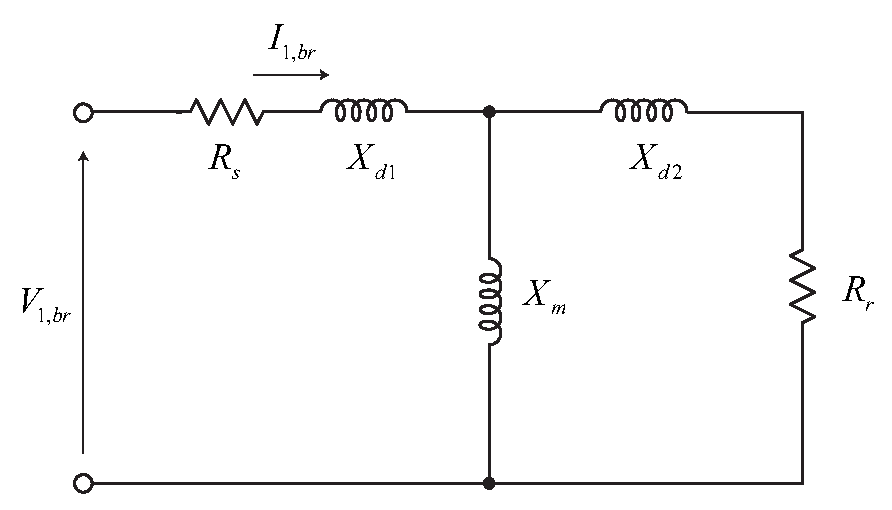
\includegraphics[width = 250pt, keepaspectratio]{figures/rotor_locked_test.eps}
	\captionsetup{width=0.5\textwidth}		
	\caption{Induction motor equivalent circuit: locked rotor conditions.}
	\label{figure:rotor_locked} 
\end{figure}
Due to condition of $R_r \ll X_m$ equations \ref{eq23} and \ref{eq24} can be reduced to
\begin{equation} \label{eq25}
	R_{br} = R_s + R_r \left(\frac{X_m}{X_m+X_{d2}}\right)^2
\end{equation} 
and 
\begin{equation} \label{eq26}
	X_{br} = X_{d1} + X_{d2} \left( \frac{X_m}{X_m+X_{d2}} \right)
\end{equation}
From the above equations the rotor resistance and leakage reactance can be found
\begin{equation} \label{eq27}
	R_{r} = \left(R_{br} - R_{s} \right) \left( \frac{X_m+X_{d2}}{X_m} \right)^2
\end{equation} \\
The performance of the motor is affected relatively little by the way in which the total total leakage reactance is distribuited between the stator and rotor and in general is taken the empirical distribution as $X_{d1} = X_{d2}$.
\begin{equation} \label{eq27}
	\left\{
	\begin{split} 
		X_{d2} = & \left(X_{br} - X_{d1}\right) \left( \frac{X_m}{X_m+X_{d1}-X_{br}} \right) \\
		X_{m} =  & X_{nl} - X_{d1}
	\end{split}\right.
\end{equation}


\subsection{Rotor resistance from steady state nominal load test}
The calculation of the rotor resistance from steady state nominal load condition is performed via equivalent circuit knowing:
\begin{itemize}
	\item Voltage input
	\item Current input
	\item Input power or shaft torque
	\item Stator frequency
	\item Rotor speed
\end{itemize}
From equivalent circuit, where all data are already calculated from the dc-measure of the stator winding, no-load test and locked-rotor test, the $I_2$ current is calculated with a preliminary underestimate value of $R_r$. Now, iteratively, for each step a small $\Delta R_r$ is add to the initial value of $R_r$ and the relative torque (as seen in equation \ref{eq17}) is calculated. The iteration stops when for a given $R_r$ the nominal torque is reached. The value of $R_r$ which gives the nominal value of torque complete the calculation of the parameters of the equivalent circuit.

\chapter{Appendix - Special Nonlinear Forms}
This appendix is taken from \cite{khalil_2}. 

The design of feedback control for nonlinear systems is simplified when the 
system takes one of certain special forms. Three such forms are presented in 
this chapter: the normal, controller and observer forms. The normal form plays 
a central role, it enables to extend to nonlinear systems some important 
results of the theory in feedback control of linear systems like minimum phase 
property when all zeros have negative real parts. For linear systems, root 
locus analysis shows that a minimum phase, relative-degree-one system can be 
stabilized by arbitrarily large feedback gain because, as gain approaches 
infinity, one branch of the root locus approaches infinity on the negative real 
axis while the remaining branches approach the zeros of the system.
\section{Normal Form}
Consider the $n$-dimensional, single-input-single-output system
\begin{flalign}
	\dot{x}&=f(x)+g(x)u \label{nf_khalil_1} \\[6pt]
	y&=h(x) \label{nf_khalil_2}
\end{flalign}
where $f$, $g$, and $h$ are sufficiently smooth in a domain $D\subset 
\mathbb{R}^n$. the mappings $f:D\rightarrow\mathbb{R}^n$ and 
$g:D\rightarrow\mathbb{R}^n$ are called vector fields on $D$. The derivative 
$\dot{y}$ is given by
\begin{flalign}
	\dot{y}=\frac{\partial h}{\partial x}\Big[f(x)+g(x)u\Big]=L_fh(x)u
\end{flalign}
where
\begin{flalign}
	L_fh(x)=\frac{\partial h}{\partial x}f(x)
\end{flalign}
is called \textit{Lie Derivative} of $h$ with respect to $x$ along $f$. The 
\textit{Lie Derivative} notion holds the following properties
\begin{flalign}
	L_gL_fh(x) &= \frac{\partial (L_fh)}{\partial x}g(x) \\[6pt]
	L_f^2h(x) &= L_fL_fh(x) = \frac{\partial (L_fh)}{\partial x}f(x) \\[6pt]
	L_f^kh(x) &= L_fL_f^{k-1}h(x) = \frac{\partial (L_f^{k-1}h)}{\partial 
	x}f(x) 
	\\[6pt]
	L_f^0h(x) &= h(x)
\end{flalign}
If $L_gh(x)=0$, then $\dot{y}=L_yh(x)$ is independent of $u$. Calculating the 
second derivative of $y$ it follows
\begin{flalign}
	y^{(2)}=\frac{\partial (L_fh)}{\partial 
	x}\Big[f(x)=g(x)u\Big]=L_f^2h(x)+L_gL_fh(x)u
\end{flalign}
If $L_gL_fh(x)u=0$, then $y^{(2)} = L_f^2h(x)$ is independent of $u$. Repeating 
this process, $h(x)$ satisfies
\begin{flalign}
	L_gL_f^{k-1}h(x)=0,\quad\text{for } i=1,2,\dots,\rho-1,\quad\text{and} 
	L_gL_f^{\rho-1}h(x)\ne0
\end{flalign}
for some integer $\rho$, then $u$ does not appear in the equations of $y,\ 
\dot{y},...,y^{(\rho-1)}$ and appears in the equation of $y^{(\rho)}$ with a 
nonzero coefficient:
\begin{flalign}
	y^{(\rho)} = L_f^\rho h(x)+ L_gL_f^{(\rho-1)}h(x)u
\end{flalign}
Such integer $\rho$ has to be less than or equal to $n$, and is called the 
\textit{relative degree} of the system, according to the following definition.

\begin{defn}
	The nonlinear system \eqref{nf_khalil_1}--\eqref{nf_khalil_2} has relative 
	degree $\rho$, $1\le\rho\le n$, in an open set $\mathcal{R}\subset D$ if, 
	for all $x\in\mathcal{R}$,
	\begin{flalign}
		L_gL_f^{i-1}h(x) = 0,\quad\text{for } i=1,2,\dots,\rho-1;\quad 
		L_gL_f^{\rho-1}h(x)\ne0
	\end{flalign}
\end{defn}
If a system has relative degree $\rho$, then its input-output map can be 
converted into a chain of integrator $y^{(\rho)}=v$ by the state feedback 
control
	\begin{flalign}
	u=\frac{1}{L_gL_f^{(\rho-1)}h(x)}\Big(-L_f^\rho h(x)+v\Big)
	\end{flalign}
\begin{example} \label{example_vanderpol_1}
Consider the controlled van der Pol equation
	\begin{flalign*}
		\dot{x}_1 &= \frac{x_2}{\epsilon} \\[6pt]
		\dot{x}_2 &= \epsilon\Big[-x_1+x_2-\frac{1}{3}x_2^3 + u\Big]
	\end{flalign*}
with output $y=x_1$. Calculating the derivatives of the output, we obtain
	\begin{flalign*}
		\dot{y} &= \dot{x}_1=\frac{x_2}{\epsilon} \\[6pt]
		\ddot{y} &= \frac{\dot{x}_2}{\epsilon} = -x_1 +x_2-\frac{1}{3}x_2^3+u
	\end{flalign*}
Hence, the system has relative degree two in $\mathbb{R}^2$. For the output 
$y=x_2$, 
 	\begin{flalign*}
 	\dot{y} &= \epsilon\Big[-x_1 +x_2-\frac{1}{3}x_2^3+u\Big] 
 \end{flalign*}
and the system has relative degree one in $\mathbb{R}^2$. For the output 
$y=\frac{1}{2}\Big(\epsilon^2x_1^2+x_2^2\Big)$,
\begin{flalign*}
	\dot{y} &= \epsilon^2x_1\dot{x}_1+x_2\dot{x}_2=\epsilon x_1x_2+\epsilon 
	x_2\Big[-x_1+x_2-\frac{1}{3}x_2^3+u\Big] = \epsilon 
	x_2^2-\frac{\epsilon}{3}x_2^4+\epsilon x_2 u
\end{flalign*}
and the system has relative degree one in $\{x_2\ne 0\}$. \hfill $\triangle$
\end{example}

\begin{example} Consider a linear system represented by the transfer function
	\begin{flalign*}
	H(s)=\frac{b_ms^m+b_{m-1}s^{m-1}+\cdots+b_0}{s^n+a_{n-1}s^{n-1}+\cdots+a_0}=\frac{N(s)}{D(s)}
	\end{flalign*}
where $m\le n$ and $b_m\ne 0$. A state model of the system can be taken as 
	\begin{flalign*}
		\dot{x}&=Ax+Bu \\[6pt]
		y&=Cx
	\end{flalign*}
where
\begin{flalign*}
	A&=\begin{bmatrix}
		0&1&0&\dots& & &\dots&0 \\[6pt]
		0&0&1&\dots& & &\dots&0 \\[6pt]
		\vdots& &\ddots& & & & &\vdots \\[6pt]
		 & & &\ddots& & & & \\[6pt]
		 & & & &\ddots& & &\vdots \\[6pt]
		 \vdots& & & & &\ddots& &0 \\[6pt]
		 0& & & & & &0&1 \\[6pt]
		 -a_0&-a_1&\dots&\dots&-a_m&\dots&\dots&-a_{n-1}
	\end{bmatrix}, \quad
	B=\begin{bmatrix}
		0 \\[6pt]
		0 \\[6pt]
		\vdots \\[6pt]
		 \\[6pt]
		 \\[6pt]
		\vdots \\[6pt]
		0 \\[6pt]
		1 \\[6pt]
	\end{bmatrix} \\[12pt]
C&=\begin{bmatrix}
	b_0&b_1&\dots&\dots&b_m&0&\dots&0 \end{bmatrix}
\end{flalign*}
This linear state model is a special case of 
\eqref{nf_khalil_1}--\eqref{nf_khalil_2}, where $f(x)=Ax$, $g(x)=B$, and 
$h(x)=Cx$. To check the relative degree of the system, we calculate the 
derivatives of the output. The first derivative is
\begin{flalign*}
	\dot{y}=CAx+CBu
\end{flalign*}
If $m=n-1$, then $CB=b_{n-1}\ne 0$ and the system has relative degree one. 
Otherwise, $CB=0$ and we continue to calculate the second derivative $y^{(2)}$. 
Noting that $CA$ is a row vector obtained by shifting the element of $C$ one 
position to the right, while $CA^2$ is obtained by shifting the elements of $C$ 
two positions to the right, and so on we see that
\begin{flalign*}
	CA^{i-1}B=0,\quad\text{for }i=1,2,\dots,n-m-1,\quad\text{and 
	}CA^{n-m-1}B=b_m\ne 0
\end{flalign*}
Thus, $u$ appears first in the equation of $y^{(n-m)}$, given by
\begin{flalign*}
	y^{(n-m)} = CA^{n-m}x+CA^{n-m-1}Bu
\end{flalign*}
and relative degree $\rho=n-m$.  \hfill $\triangle$
\end{example}
Concerning the previous example, consider the Euclidean division 
\begin{flalign}
	D(s)=Q(s)N(s)+R(s)
\end{flalign}
where $Q(s)$ and $R(s)$ are the quotient and remainder polynomials, 
respectively. From Euclidean division rules, we know that $\deg Q=n-m=\rho$, 
$\deg R<m$, and the leading coefficient of $Q(s)$ is $1/b_m$. With this 
representation of $D(s)$, we can rewrite $H(s)$ as follows
\begin{flalign}
	H(s)=\frac{N(s)}{Q(s)N(s)+R(s)}=\frac{\frac{1}{Q(s)}}{1+\frac{1}{Q(s)}\frac{R(s)}{N(s)}}
\end{flalign}
Thus, $H(s)$ can be represented as a negative feedback connection with $1/Q(s)$ 
in the forward path and $R(s)/N(s)$ in the feedback path, see 
Figure~\ref{khalil_fig_1}. 
\begin{figure}[H]
	\centering
	\includegraphics[width = 200pt, angle = 0, 
	keepaspectratio]{figures/feedback_representation_of_hs_1.eps}
	\captionsetup{width=0.5\textwidth}	
	\caption{Feedback representation of $H(s)$.}
	\label{khalil_fig_1}
\end{figure}
The $\rho$th-oder transfer function $1/Q(s)$ has no 
zeros and can be realized by the $\rho$th-dimensional state vector 
$\xi=\begin{bmatrix}y&\dot{y}&\dots&y^{(\rho-1)}\end{bmatrix}^T$ to obtain the 
state model
\begin{flalign}
	\dot{\xi}&=\Big(A_c+B_c\lambda^T\Big)\xi+B_cb_me \\[6pt]
	y&=C_c\xi
\end{flalign}
where $\Big(A_c,\ B_c,\ C_c\Big)$ is a canonical for representation of a chain 
of $\rho$ integrators,
\begin{flalign*}
	A_c&=\begin{bmatrix}
		0&1&0&\dots&0 \\[6pt]
		0&0&1&\dots&0 \\[6pt]
		\vdots& &\ddots& &\vdots \\[6pt]
		\vdots& & &0&1 \\[6pt]
		0&0&0&0&0
	\end{bmatrix}_{\rho\times\rho} \quad
	B_c=\begin{bmatrix}
		0 \\[6pt]
		0 \\[6pt]
		\vdots \\[6pt]
		0 \\[6pt]
		1 \\[6pt]
	\end{bmatrix} \quad
	C_c=\begin{bmatrix}1&0&\dots&0&0 \end{bmatrix}
\end{flalign*}
and $\lambda\in\mathbb{R}^\rho$. Let
\begin{flalign}
	\dot{\eta}&=A_0\eta+B_0y \\[6pt]
	w&=C_0\eta
\end{flalign}
be a (minimal realization) state model of $R(s)/N(s)$. The eigenvalues of $A_0$ 
are the zeros of the polynomial $N(s)$, which are the zeros of the transfer 
function $H(s)$. From the feedback connection, we see that $H(s)$ can be 
realized by the state model
\begin{flalign}
	\dot{\eta}&=A_0\eta+B_0C_c\xi \label{nf_khalil_3} \\[6pt]
	\dot{\xi}&=A_c\xi+B_c\Big(\lambda^T\xi-b_mC_0\eta+b_mu\Big) 
	\label{nf_khalil_4} \\[6pt]
	y&=C_c\xi \label{nf_khalil_5}
\end{flalign}

The next task is to develop a nonlinear version of the state 
model~\eqref{nf_khalil_3}--\eqref{nf_khalil_5} for the 
system~\eqref{nf_khalil_1}--\eqref{nf_khalil_2} when it has relative degree 
$\rho$. Equivalently, a change of variable $z=T(x)$ will be found such that the 
new state $z$ can be partitioned into a $\rho$-dimensional vector $\xi$ and 
$(n-\rho)$-dimensional vector $\eta$, where the components of $\xi$ comprise 
the output and its derivatives up to $y^{(\rho-1)}$, while $\eta$ satisfies a 
differential equation whose right-hand side depends on $\eta$ and $\xi$, but 
not on $u$. $\xi$ is selected as in the linear case:
\begin{flalign}
	\xi = \begin{bmatrix} y \\[6pt] y^{(1)} \\[6pt] \vdots \\[6pt] y^{(\rho-1)} 
	\end{bmatrix} = \begin{bmatrix} h(x) \\[6pt] L_fh(x) \\[6pt] \vdots \\[6pt] 
	L_f^{(\rho-1)}h(x)	\end{bmatrix}
\end{flalign}
 when $\rho=n$, there is no $\eta$ variable and the change of variables is 
 given by
 \begin{flalign}\label{nf_khalil_6}
 	z=T(x) = \begin{bmatrix} h(x) & L_fh(x) & \cdots & 
 		L_f^{(n-1)}h(x)	\end{bmatrix}^T
 \end{flalign}
 when $\rho<n$, the change of variables is as follows
  \begin{flalign}\label{nf_khalil_7}
 	z=T(x) = \begin{bmatrix} \phi_1(x) \\[6pt] \vdots \\[6pt] 
 	\phi_1^{n-\rho}(x) \\[6pt] h(x) \\[6pt] \vdots \\[6pt] 
 		L_f^{(\rho-1)}h(x)	\end{bmatrix} =
 	\begin{bmatrix} \phi(x) \\[6pt] \mathcal{H}(x)	\end{bmatrix}=
 	\begin{bmatrix} \eta \\[6pt] \xi	\end{bmatrix}
 \end{flalign}
where $\phi_1$ to $\phi_{n-\rho}$ are chosen such that $T(x)$ is a 
diffeomorphism on a domain $D_x\subset\mathcal{R}$ and
\begin{flalign}\label{nf_khalil_8}
	\frac{\partial\phi_i}{\partial x}g(x) = 0,\quad\text{for }1\le i \le 
	n-\rho, \forall x\in D_x
\end{flalign}
so that the $u$ term cancels out in
\begin{flalign}
	\dot{\eta}=\frac{\partial \phi}{\partial}\Big[f(x)+g(x)u\Big]
\end{flalign}
The next theorem shows that the change of 
variables~\eqref{nf_khalil_6}--\eqref{nf_khalil_7} is well defined at least 
locally.
\begin{thm}\label{nf_khalil_thm_1}
	Consider the system~\eqref{nf_khalil_1}--\eqref{nf_khalil_2} and suppose it 
	has relative degree $\rho\le n$ in $\mathcal{R}$. If $\rho=n$, then for 
	every $x_0\in\mathcal{R}$, a neighbourhood N of $x_0$ exists such that 
	the map $T(x)$ of~\eqref{nf_khalil_6}, restrict to N, is a diffeomorphism 
	on N. If $\rho < n$, then, for every $x_0\in\mathcal{R}$, a neighbourhood N 
	of $x_0$ and continuously differentiable functions 
	$\phi_1(x),\dots,\phi_{n-\rho}$ exist such that~\eqref{nf_khalil_8} is 
	satisfied for all $x\in N$ and the map $T(x)$ of~\eqref{nf_khalil_7}, 
	restricted to N, is a diffeomorphism on N. \hfill $\square$
\end{thm}

when $\rho < n$, the change of variables~\eqref{nf_khalil_7} 
transform~\eqref{nf_khalil_1}--\eqref{nf_khalil_2} into
\begin{flalign}
	\dot{\eta}&=f_0(\eta,\xi) \label{nf_khalil_9} \\[6pt]
	\dot{\xi}&=A_c\xi+B_c\Big[L_f^\rho h(x) +L_gL_f^{\rho-1}h(x)u\Big] 
	\label{nf_khalil_10} \\[6pt]
	y&=C_c\xi \label{nf_khalil_11}
\end{flalign}
where $\xi\in\mathscr{R}^\rho$, $\eta\in\mathbb{R}^{n-\rho}$, $\Big(Ac,\ B_c,\ 
C_c\Big)$ is a canonical form representation of a chain of $\rho$ integrators, 
and
 \begin{flalign}\label{nf_khalil_12}
 	f_0(\eta,\xi) = \frac{\partial \phi}{\partial x}f(x)\Bigg|_{x=T^{-1}(z)}
 \end{flalign}
We have kept $L_f^\rho h$ and $L_gL_f^{\rho-1}h$ in~\eqref{nf_khalil_10} as function of $x$ because they are independent of the choice of $\phi$. When expressed in the new coordinates~\eqref{nf_khalil_10} is given by
\begin{equation}
	\dot{\xi}=A_c\xi+B_c\big[\tilde{\psi}(\eta,\xi)+\tilde{\gamma}(\eta,\xi)u\big]
\end{equation}
where 
\begin{equation}
	\tilde{\psi}(\eta,\xi)=L_f^\rho h(x)\Big|_{x=T^{-1}(z)}\quad\quad \tilde{\gamma}(\eta,\xi)=L_gL_f^{\rho-1}h(x)
\end{equation}
If $x^*$ is an open-loop equilibrium point of~\eqref{nf_khalil_1}, then $(\eta^*,\,\xi^*)$, defined by
\begin{equation}
	\eta^*=\phi(x^*),\quad\xi^*=\begin{bmatrix}
		h(x^*) & 0 & \dots & 0
	\end{bmatrix}
\end{equation}
is an equilibrium point of~\eqref{nf_khalil_9}--\eqref{nf_khalil_11}. If $h(x^*)=0$, we can transformer $x^*$ into the origin point $(\eta=0,\,\xi=0)$ by choosing $\phi(x)$ such that $\phi(x^*)=0$, which is always possible because adding a constant to a function $\phi_i$ that satisfies~\eqref{nf_khalil_8} does not alter this condition, nor the property that $T(x)$ is a diffeomorphism.

Equations~\eqref{nf_khalil_9}--\eqref{nf_khalil_11} are said to be in the \textit{normal form}. This form decomposes the system into internal dynamics~\eqref{nf_khalil_9} and external dynamics~\eqref{nf_khalil_10}--\eqref{nf_khalil_11}. The state feedback control
\begin{equation*}
 u=\frac{1}{L_gL_f^{\rho-1}}\Big[-L_f^\rho h(x)+v\Big]
\end{equation*}
converts the external dynamics into a chain of $\rho$ integrators, $y^{(\rho)}=v$, and makes the internal dynamics unobservable from the output $y$. When $y(t)$ is identically zero, so is $\xi(t)$. Setting $\xi=0$ in \eqref{nf_khalil_10} results in
\begin{equation}\label{nf_khalil_13}
	\dot{\eta}=f_0(\eta,0)
\end{equation}
which is called the \textit{zero dynamics}. The system is said to be \textit{minimum phase} if~\eqref{nf_khalil_13} has an asymptotically stable equilibrium point in the domain of interest. In particular, if $T(x)$ is chosen such that the origin $(\eta=0,\,\xi=0)$ is an equilibrium point of~\eqref{nf_khalil_9}--\eqref{nf_khalil_11}, then the system is minimum phase if the origin of the zero dynamics~\eqref{nf_khalil_13} is asymptotically stable. It is useful to know that the zero dynamics can be characterized in the original coordinates. Noting that
\begin{equation*}
	y(t)=0\Rightarrow\xi(t)=0\Rightarrow u(t)=-\frac{L_f^\rho h(x(t))}{L_gL_f^{\rho-1}h(x(t))}
\end{equation*}
we see that if the output is identically zero, the solution of the state equation must be confined to the set
\begin{equation*}
	\mathscr{Z}^*=\big\{ x\in\mathscr{R}|h(x)=L_fh(x)=\dots=L_f^{\rho-1}h(x)=0\big\}
\end{equation*}
and the input must be
\begin{equation*}
	u=u^*(x)\stackrel{\text{def}}{=}-\frac{L_f^\rho h(x)}{L_gL_f^{\rho-1}h(x)}\Big|_{x\in\mathscr{Z}^*}
\end{equation*}
The restricted motion of the system is described by
\begin{equation*}
	\dot{x}=f^*(x)\stackrel{\text{def}}{=}\Big[f(x)-g(x)\frac{L_f^\rho h(x)}{L_gL_f^{\rho-1}h(x)}\Big]_{x\in\mathscr{Z}^*}
\end{equation*}
In the special case, the system has no zero dynamics and, by default, is said to be minimum phase.
\begin{example}
	Consider the controlled van der Pol equation
	\begin{flalign*}
		\dot{x}_1 = \frac{x_2}{\epsilon},\qquad
		\dot{x}_2 = \epsilon\Big[-x_1+x_2-\frac{1}{3}x_2^3 + u\Big],\qquad
		y=x_2
	\end{flalign*}
We have seen in Example~\ref{example_vanderpol_1} that the system has relative degree one in $\mathbb{R}^2$. Taking $\xi=y$ and $\eta=x_1$, we see that the system is already in the normal form. The zero dynamics are given by the equation $\dot{x}_1=0$, which does not have an asymptotically stable equilibrium point. Hence, the system is not minimum phase. 

	\hfill $\triangle$
\end{example}
\begin{example}
	The system
	\begin{equation*}
	\begin{aligned}
		\dot{x}_1=-x_1+\frac{2+x_3^2}{1+x_3^2}u,\qquad
		\dot{x}_2=x_3,\qquad
		\dot{x}_3=x_1x_3+u,\qquad
		y=x_2
	\end{aligned}
	\end{equation*}
	has an open-loop equilibrium point at the origin, The derivatives of the output are
	\begin{equation*}
	\begin{aligned}
		\dot{y}&=\dot{x}_2=x_3 \\[6pt]
		\ddot{y}&=\dot{x}_3=x_1x_3+u
	\end{aligned}
	\end{equation*}	
	Therefore, the system has relative degree two in $\mathbb{R}^3$. To characterize the zero dynamics, restrict $x$ to $\mathscr{Z}^*=\{x_2=x_3=0\}$ and take
	\begin{equation*}
		u=u^*(x)=-\frac{L_f^2h(x)}{L_gL_fh(x)}\Big|_{x\in\mathscr{Z}^*}=-x_1x_3\Big|_{x\in\mathscr{Z}^*}=0
	\end{equation*}
	This process yields $\dot{x}_1=-x_1$, which shows that the system is minimum phase. To transform the system into the normal form, we choose $\phi(x)$ such that 
	\begin{equation*}
		\phi(0)=0,\quad\frac{\partial \phi}{\partial x}g(x)=0
	\end{equation*}
	and $T(x)=\begin{bmatrix} \phi(x)&x_2&x_3 \end{bmatrix}^T$ is a diffeomorphism on some domain containing the origin. The partial differential equation
	\begin{equation*}
		\Bigg[\frac{\partial \phi}{\partial x_1}\Bigg]\frac{2+x_3^2}{1+x_3^2}+\frac{\partial \phi}{\partial x_3}=0,\qquad\phi(0)=0
	\end{equation*}
	can be solved by separation of variables to obtain $\phi(x)=x_1-x_3-\tan^{-1}x_3$. The mapping $T(x)$ is a global diffeomorphism because it is proper and $\big[\partial T/\partial x\big]$ is nonsingular for all $x$. Thus, the normal form
	\begin{equation*}
		\begin{aligned}
			\dot{\eta} &= -(\eta+\xi_2+\tan^{-1}\xi_2)\Big(1+\frac{2+\xi_2^2}{1+\xi_2^2}\xi_2\Big) \\[6pt]
			\dot{\xi}_1 &= \xi_2 \\[6pt]
			\dot{\xi}_2 &= (\eta+\xi_2+\tan^{-1}\xi_2)\xi_2+u\\[6pt]
			y&=\xi_1
		\end{aligned}
	\end{equation*}
	is defined globally.
		
	\hfill $\triangle$
\end{example}

\section{Controller Form}
A nonlinear system is in controller form if its state model is given by
\begin{flalign}
	\dot{x}=Ax+B\Big[\psi(x)+\gamma(x)u\Big] \label{nf_khalil_15}
\end{flalign}
where $(A,\,B)$ is controllable and $\gamma(x)$ is a nonsingular matrix for all $x$ in the domain of interest. The system~\eqref{nf_khalil_15} can be converter into the controllable linear system
\begin{flalign*}
	\dot{x}=Ax+Bv
\end{flalign*}
by the state feedback control
\begin{flalign*}
	u=\gamma^{-1}(x)\Big[-\psi(x)+v\Big]
\end{flalign*}
where $\psi^{-1}(x)$ is the inverse matrix of $\gamma(x)$. Therefore, any system that can be represented in the controller form is said to be \textit{feedback linearizable}.
\begin{example}
	An $m$-link robot is modeled by
	\begin{equation*}
		\dot{x}_1=x_2,\qquad\dot{x}_2=M^{-1}(x_1)\Big[u-C(x_1,x_2)x_2-Dx_2-g(x_1)\Big]
	\end{equation*}
	Taking $x=\begin{bmatrix} x_1&x_2\end{bmatrix}^T$ the state model takes the form~\eqref{nf_khalil_15} with
	\begin{equation*}
		A=\begin{bmatrix} 0 & I_m \\[6pt] 0 & 0 \end{bmatrix},\quad B=\begin{bmatrix} 0 \\[6pt] I_m\end{bmatrix},\quad \psi=-M^{-1}(Cx_2+Dx_2+g),\quad\gamma=M^{-1}
	\end{equation*}
	
		\hfill $\triangle$
\end{example}
Even if the state model is not in the controller form, the system will be feedback linearizable if it can be transformed into that form. In this section, we characterize the class of feedback linearizable single-input systems
\begin{equation}\label{nf_khalil_16}
	\dot{x}=f(x)+g(x)u
\end{equation}
where $f$ and $g$ are sufficiently smooth vector fields on a domain $D\subset\mathbb{R}^n$. From the previous section we see that the system~\eqref{nf_khalil_16} is feedback linearizable in a neighbourhood of $x_0\in D$ if a (sufficiently smooth) function $h$ exists such that the system
 \begin{equation}\label{nf_khalil_17}
 	\dot{x}=f(x)+g(x)u,\qquad y=h(x)
 \end{equation}
has relative degree $n$ in a neighbourhood of $x_0$. Theorem~\ref{nf_khalil_thm_1} ensures that the map 
\begin{equation*}
	T(x)=\begin{bmatrix} h(x) & L_fh(x) & \dots & L_f^{n-1}h(x)	\end{bmatrix}
\end{equation*}
restricted to a neighbourhood $N$ of $x_0$, is a diffeomorphism on $N$ and the change of variables $z=T(x)$ transforms the system into the normal form
\begin{equation*}
	\dot{z}=A_cz+B_c\Big[\tilde{\psi}(z) + \tilde{\gamma}(z)u\Big],\qquad y=C_cz
\end{equation*}
where $(Ac,\,B_c,\,C_c)$ is a canonical form representation of a chain of $n$-integrators. On the other hand, if~\eqref{nf_khalil_16} is feedback linearizable in a neighbourhood $N$ of $x_0\in D$, then there is a change of variables $\zeta=S(x)$ that transform the system into 
\begin{equation*}
	\dot{\zeta}=A\zeta+B\Big[\bar{\psi}(\zeta)+\bar{\gamma}(\zeta)u\Big]
\end{equation*}
where $(A,\,B)$ is controllable and $\bar{\gamma}(\zeta)\ne0$ in $S(N)$. For any controllable pair $(A,\,B)$, we can find a nonsingular matrix $M$ that transforms $(A,\,B)$ into the controllable canonical form:
\begin{equation*}
	MAM^{-1}=A_c+B_c\lambda^T,\qquad MB=B_c
\end{equation*}
The change of variables 
\begin{equation*}
	z=M\zeta=MS(x)\stackrel{\text{def}}{=}T(x)
\end{equation*}
transform~\eqref{nf_khalil_16} into
\begin{equation*}
	\dot{z} = A_cz+B_c\Big[\tilde{\psi}(z)+\tilde{\gamma}(z)u\Big]
\end{equation*}
where $\tilde{\gamma}(z)=\bar{\gamma}(M^{-1}z)$ and $\tilde{\psi}(z)=\bar{\psi}(M^{-1}z)+\lambda^Tz$.

In summary the system~\eqref{nf_khalil_16} is feedback linearizable in a 
neighbourhood of $x_0\in D$ if and only if a (sufficiently smooth) function 
$h(x)$ exists such that the system~\eqref{nf_khalil_17} has relative degree $n$ 
in a domain $D_x\subset D$, with $x_0\in D_x$, or, equivalently, $h$ satisfies 
the partial differential equations
\begin{equation}\label{nf_khalil_18}
	L_gL_f^{i-1}h(x) = 0,\qquad i=1,2,\dots,n-1
\end{equation} 
subject to the condition
\begin{equation}\label{nf_khalil_19}
	L_gL_f^{n-1}h(x) \ne 0
\end{equation} 
for all $x\in D_x$. The existence of $h$ can be characterized by necessary and 
sufficient conditions on the vector fields $f$ and $g$. These conditions use 
the notion of \textit{Lie brackets} and \textit{involutive distributions}, 
which we introduce next.

For two vectors fields $f$ and $g$ on $D\subset\mathbb{R}^n$, the \textit{Lie 
brackets} $[f,g]$ is a third vector field defined by
\begin{equation}
[f,g]=\frac{\partial g}{\partial x}f(x)-\frac{\partial f}{\partial x}g(x)
\end{equation} 
where $[\partial f/\partial x]$ and $[\partial f/\partial x]$ are Jacobian 
matrices. The Lie bracket $[f,g](x)$ is invariant under the change of variables 
$z=T(x)$ in the sense that if
\begin{equation}
	\tilde{f}(z)=\frac{\partial T}{\partial 
	x}f(x)\Bigg|_{x=T^{-1}(z)}\quad\text{and}\quad 
	\tilde{g}(z)=\frac{\partial T}{\partial x}g(x)\Bigg|_{x=T^{-1}(z)}
\end{equation}
then
\begin{equation}
	[\tilde{f},\tilde{g}](z)=\frac{\partial T}{\partial 
		x}[{f},{g}](x)\Bigg|_{x=T^{-1}(z)}
\end{equation}
We may repeat bracketing of $g$ with $f$. The following notation is used to 
simplify this process:
\begin{equation*}
	\begin{aligned}
			ad_f^0g(x)&=g(x) \\[6pt]
			ad_fg(x)&=[f,g](x) \\[6pt]
			ad_f^kg(x)&=[f,ad_f^{k-1}g](x),\quad k\ge1
	\end{aligned}
\end{equation*}
It is obvious that $[f,g]=-[g,f]$ and for constant vector fields $f$ and $g$, 
$[f,g]=0$.
\begin{example}
	Let
	\begin{equation*}
		f(x) = \begin{bmatrix} x_2 \\[6pt] -\sin x_1 - x_2 
		\end{bmatrix},\quad		g(x)=\begin{bmatrix} 0 \\[6pt] x_1 
		\end{bmatrix}
	\end{equation*}
	Then,
	\begin{flalign*}
		[f,g] &= \begin{bmatrix} 0 & 0 \\[6pt] 1 & 0 \end{bmatrix} 
		\begin{bmatrix} x_2 \\[6pt] -\sin x_1 - x_2 \end{bmatrix}- 
		\begin{bmatrix} 0 & 1 \\[6pt] -\cos x_1 - 1 \end{bmatrix}
		\begin{bmatrix} 0 \\[6pt] x_1 \end{bmatrix} \\[6pt]
		&= \begin{bmatrix} -x_1 \\[6pt] x_1+x_2 \end{bmatrix} 
		\stackrel{\text{def}}{=} ad_fg
	\end{flalign*}
	\begin{flalign*}
		[f,ad_fg] &= \begin{bmatrix} -1 & 0 \\[6pt] 1 & 1 \end{bmatrix} 	
		\begin{bmatrix} x_2 \\[6pt] -\sin x_1 - x_2 \end{bmatrix}- 
		\begin{bmatrix} 0 & 1 \\[6pt] -\cos x_1 - 1 \end{bmatrix}
		\begin{bmatrix} -x_1 \\[6pt] x_1+x_2 \end{bmatrix} \\[6pt]
		&= \begin{bmatrix} -x_1-2x_2 \\[6pt] x_1+x_2-\sin x_1-x_1\cos x_1 
		\end{bmatrix} \stackrel{\text{def}}{=} ad_f^2g
	\end{flalign*}

	\hfill$\triangle$
\end{example}
\begin{example}
	If $f(x)=Ax$ and $g$ is a constant vector field, then 
	\begin{flalign*}
	ad_fg&=[f,g]=-Ag	\\[6pt]
	ad^2_fg&=[f,ad_fg]=-A(-Ag)=A^2g \\[6pt]
	ad_f^kg&=(-1)^kA^kg
	\end{flalign*} 
	
	\hfill$\triangle$
\end{example}

For vectors fields $f_1,\,f_2,\dots,f_k$ on $D\subset\mathbb{R}^n$, let
\begin{equation*}
	\Delta(x)=\spn\{f_1(x),\,f_2(x), \dots,f_k(x)\}
\end{equation*}
be the subspace of $\mathbb{R}^n$ spanned by the vectors 
$f_1(x),\,f_2(x),\,\dots,f_k(x)$ at any fixed $x\in D$. The collection of 
all 
vector spaces $\Delta(x)$ for $x\in D$ is called a distribution and referred 
to 
by
\begin{equation*}
	\Delta = \spn\{f_1,\,f_2,\dots,f_k\}
\end{equation*}
The dimension of $\Delta(x)$, defined by
\begin{equation*}
	\dim(\Delta(x))=\rank\Big[f_1(x),\,f_2(x),\dots,f_k(x)\Big]
\end{equation*}
may vary with $x$, but if $\Delta=\spn\{f_1,\dots,f_k\}$, where 
$\{f_1(x),\dots,f_k(x)\}$ are linearly independent for all $x\in D$, then 
$\dim(\Delta(x))=k$ for all $x\in D$. In this case, we say that $\Delta$ is 
a 
nonsingular distribution on $D$, generated by $f_1,\dots,f_k$. A 
distribution $\Delta$ is \textit{involutive} if
\begin{equation*}
	g_1\in\Delta\quad\text{and}\quad g_2\in\Delta\Rightarrow\big[g_1,\,g_2\big]\in\Delta
\end{equation*}
If $\Delta$ is a nonsingular distribution on $D$, generated by $f_1,\dots,f_k$, then $\Delta$ is involutive if and only if
\begin{equation*}
	[f_i,\,f_j]\in \Delta,\qquad\forall\quad 1\le i,j\le k
\end{equation*}
One dimensional distributions, $\Delta=\spn\{f\}$, and distributions generated by constant vector fields are always involutive.
\begin{example}
	Let $D=\mathbb{R}^3$ and $\Delta =\spn\{f_1,\,f_2\}$, where
	\begin{equation*}
		f_1=\begin{bmatrix} 2x_2 \\[6pt] 1 \\[6pt] 0 \end{bmatrix},\qquad
		f_2=\begin{bmatrix} 1 \\[6pt] 0 \\[6pt] x_2 \end{bmatrix}
	\end{equation*}
	It can be verified that $\dim(\Delta(x))=2$ for all $x$. The Lie bracket $[f_1,\,f_2]\in\Delta$ if and only if rank $\Big[f_1(x),\,f_2(x),\,[f_1,\,f_2](x)\Big]=2$, for all $x\in D$. However,
	\begin{equation*}
		\rank\Big[f_1(x),\,f_2(x),\,[f_1,\,f_2](x)\Big]=\rank\begin{bmatrix} 2x_2 & 1 & 0 \\[6pt] 1 & 0 & 0 \\[6pt] 0 & x_2 & 1	\end{bmatrix}=3,\qquad\forall x\in D
	\end{equation*}
Hence, $\Delta$ is not involutive.
	\hfill$\triangle$
\end{example}
\begin{example}
	Let $D=\{x\in\mathbb{R}^3\,|\,x_1^2+x_3^2\ne0\}$ and $\Delta=\spn\{f_1\,f_2\}$, where
	\begin{equation*}
		f_1=\begin{bmatrix} 2x_3 \\[6pt] -1 \\[6pt] 0 \end{bmatrix},\qquad
		f_2=\begin{bmatrix} -x_1 \\[6pt] -2x_2 \\[6pt] x_3 \end{bmatrix}
	\end{equation*}
	It can be verified that $\dim(\Delta(x))=2$ for all $x\in D$ and
	\begin{equation*}
		\rank\Big[f_1(x),\,f_2(x),\,[f_1,\,f_2](x)\Big]=\rank\begin{bmatrix} 2x_3 & -x_1 & -4x_3 \\[6pt] -1 & -2x_2 & 2 \\[6pt] 0 & x_3 & 0	\end{bmatrix}=2,\qquad\forall x\in D
	\end{equation*}
Therefore, $[f_1,\,f_2]\in\Delta$. Since $[f_2,\,f_1]=-[f_1,\,f_2]$, $\Delta$ is involutive.
		\hfill$\triangle$
\end{example}
We are now ready to characterize the class of feedback linearizable systems.
\begin{thm}\label{involutive_thm}
	The system~\eqref{nf_khalil_16} is feedback linearizable in a neighbourhood of $x_0\in D$ if and only if there is a domain $D_x\subset D$, with $x_0\in D_x$, such that
	\begin{enumerate}
		\item the matrix $\mathscr{G}(x)=[g(x),\,ad_fg(x),\,\dots,ad_f^{n-1}g(x)]$ has rank $n$ for all $x\in D_x$;
		\item the distribution $\mathscr{D}=\spn\{g,\,ad_fg,\,\dots,ad_f^{n-2}\}$ is involutive in $D_x$.
	\end{enumerate}
	
		\hfill$\square$
\end{thm}

The conditions of the theorem ensure that for each $x_0\in D$ there is a function $h(x)$ satisfying~\eqref{nf_khalil_18}--\eqref{nf_khalil_19} in some neighbourhood $N$ of $x_0$ and the system is feedback linearizable in $N$. They do not guarantee feedback linearizability in a given domain. However, as we solve the partial differential equations~\eqref{nf_khalil_18} for $h(x)$, it is usually possible to determine a domain $D_x$ in which the system is feedback linearizable. This point is illustrated in the next three examples. In all examples, we assume that the system~\eqref{nf_khalil_16} has an equilibrium point $x^*$ when $u=0$, and choose $h(x)$ such that $h(x^*)=0$. Consequently, $z=T(x)$ maps $x=x^*$ into $z=0$.
\begin{example}
Consider the system
	\begin{equation*}
		\dot{x}=\begin{bmatrix} a\sin x_2 \\[6pt] -x_1^2 \end{bmatrix} + \begin{bmatrix} 0 \\[6pt] 1 \end{bmatrix}u\stackrel{\text{def}}{=}f(x)+gu
	\end{equation*}
We have
	\begin{equation*}
		ad_fg=[f,g]=-\frac{\partial f}{\partial x}g = \begin{bmatrix} -a\cos x_2 \\[6pt] 0 \end{bmatrix}
	\end{equation*}
The matrix
	\begin{equation*}
		[g,ad_fg]= \begin{bmatrix} 0 &-a\cos x_2 \\[6pt] 1 & 0 \end{bmatrix}
	\end{equation*}	
has rank two for all $x$ such that $\cos x_2\ne0$. The distribution $\spn\{g\}$ is involutive. Hence, the conditions of Theorem~\ref{involutive_thm} are satisfied in the domain $D_x=\{\abs{x}<\pi/2\}$. The find the change of variables that transform the system into the form~\eqref{nf_khalil_15}, we want to find $h(x)$ that satisfies
\begin{equation*}
	\frac{\partial h}{\partial x}g=0,\quad\frac{\partial L_fh}{\partial x}g\ne0,\quad\text{and}\quad h(0)=0
\end{equation*}
From the condition $[\partial h/\partial x]g=0$, we have $[\partial h/\partial x]g=[\partial h/\partial x_2]=0$. Thus, $h$ must be independent of $x_2$. Therefore, $L_fh(x)=[\partial h/\partial x_1]a\sin x_2$. The condition
\begin{equation*}
	\frac{\partial L_fh}{\partial x}g=\frac{\partial (L_fh)}{\partial x_2}=\frac{\partial h}{\partial x_1}a\cos x_2\ne0
\end{equation*}
is satisfied in $D_x$ if $(\partial h/\partial x_1)\ne0$. The choice $h=x_1$ yields
\begin{equation}
	z = T(x) = \begin{bmatrix} x_1 \\[6pt] a\sin x_2 \end{bmatrix}
\end{equation}
and the transformed system
\begin{equation}
	\dot{z}_1=z_2,\qquad\dot{z}_2=\sqrt{a^2-z^2}(-z_1^2+u)	
\end{equation}
			is well defined for $-a<z_2<a$
			
			\hfill$\triangle$
\end{example}
\begin{example}
	A single link manipulator with flexible joints and negligible damping can be represented by the four-dimensional model
	\begin{equation*}
		\dot{x}=f(x)+gu
	\end{equation*}
	where 
	\begin{equation*}
		f(x)=\begin{bmatrix} x_2 \\[6pt] -a\sin x_1-b(x_1-x_3) \\[6pt] x_4 \\[6pt] c(x_1-x_3)
		\end{bmatrix}, \qquad 
			g=\begin{bmatrix} 0 \\[6pt] 0 \\[6pt] 0 \\[6pt] d
		\end{bmatrix}
	\end{equation*}
	and $a$, $b$, $c$, and $d$ are positive constants. The unforced has an equilibrium point at $x=0$. We have
	\begin{equation*}
		ad_fg=[f,\,g]=-\frac{\partial f}{\partial x}g=\begin{bmatrix} 0 \\[6pt] 0 \\[6pt] -d \\[6pt] 0 \end{bmatrix}, \quad
		ad_f^2g=[f,\,ad_fg]=-\frac{\partial f}{\partial x}ad_fg=\begin{bmatrix} 0 \\[6pt] bd \\[6pt] 0 \\[6pt] -cd \end{bmatrix}
	\end{equation*}
	\begin{equation*}
		ad_f^3g=[f,\,ad_f^2g]=-\frac{\partial f}{\partial x}ad_f^2g=\begin{bmatrix} -bd \\[6pt] 0 \\[6pt] cd \\[6pt] 0 \end{bmatrix}
	\end{equation*}
	The matrix
	\begin{equation*}
		[g,\,ad_fg,\,ad_f^2g,\,ad_f^3g] = \begin{bmatrix} 0&0&0&-bd \\[6pt] 0&0&bd&0 \\[6pt] 0&-d&0&cd \\[6pt] d&0&-cd&0 \end{bmatrix}
	\end{equation*}
	has full rank for all $x\in\mathbb{R}^4$. The distribution $\spn(g,ad_fg,ad^2_fg)$ is involutive since $g$, $ad_fg$, and $ad_f^2g$ are constant vector fields. Thus, the conditions of Theorem~\ref{involutive_thm} are satisfied for all $x\in\mathbb{R}^4$. To transform the system into the controller form, we want to find $h(x)$ that satisfies
	\begin{equation*}
		\frac{\partial(L_f^{i-1})}{\partial x}g=0, \quad i=1,2,3,\quad \frac{\partial(L_f^3h)}{\partial x} g\ne, \quad\text{and}\quad h(0)=0
	\end{equation*}
From the condition $[\partial h/\partial x]g=0$, we have $(\partial h/\partial x_4)=0$, so we must choose $h$ independent of $x_4$. Therefore,
\begin{equation*}
	L_fh(x) = \frac{\partial h}{\partial x_1}x_2+\frac{\partial h}{\partial x_2}[-a\sin x_1-b(x_1-x_3)]+\frac{\partial h}{\partial x_3}x_4
\end{equation*}
From the condition $[\partial (L_fh)/\partial x]g=0$, we have
\begin{equation*}
	\frac{\partial(L_fh)}{\partial x_4}=0\quad\Rightarrow\quad\frac{\partial h}{\partial x_3}=0
\end{equation*}
So, we choose $h$ independent of $x_3$. Therefore, $L_fh$ simplified to 
\begin{equation*}
	L_fh(x)=\frac{\partial h}{\partial x_1}x_2+\frac{\partial h}{\partial x_2}[-a\sin x_1-b(x_1-x_3)]
\end{equation*}
and 
\begin{equation*}
	L_f^2h(x)=\frac{\partial(L_fh)}{\partial x_1}x_2+\frac{\partial(L_fh)}{\partial x_2}[-a\sin x_1 - b(x_1-x_3)]+\frac{\partial(L_fh)}{\partial x_3}x_4
\end{equation*}
Finally,
\begin{equation*}
	\frac{\partial(L_f^2h)}{\partial x_4}=0,\quad\Rightarrow\quad\frac{\partial(L_fh)}{\partial x_3}=0\quad\Rightarrow\quad\frac{\partial h}{\partial x_2}=0
\end{equation*}
and we choose $h$ independent of $x_2$. Hence,
\begin{equation*}
	L_f^3h(x)=\frac{\partial(L_f^2h)}{\partial x_1}x_2+\frac{\partial(L_f^2h)}{\partial x_2}[-a\sin x_1-b(x_1-x_3)]+\frac{\partial(L_f^2h)}{\partial x_3}x_4
\end{equation*}
and the condition $[\partial(L_f^3h)/\partial x]g\ne0$ is satisfied whenever $(\partial f/\partial x_1)\ne0$. Therefore, we take $h(x)=x_1$. The change of variables
\begin{flalign*}
	z_1&=h(x)=x_1 \\[6pt]
	z_2&=L_fh(x)=x_2 \\[6pt]
	z_3&=L_f^2h(x)=-a\sin x_1 -b(x_1-x_3) \\[6pt]
	z_4&=L_f^3h(x)=-ax_2\cos x_1-b(x_2-x_4)
\end{flalign*}
transform the system into the controller form 
\begin{equation*}
	\begin{aligned}
		\dot{z}_1 &= z_2, \quad \dot{z}_2 = z_3,\quad \dot{z}_3 = z_4 \\[6pt]
		\dot{z}_4 &= -(a\cos z_1+b+c)z_3+a(z_2^2-c)\sin z_1+bdu
\end{aligned}
\end{equation*}
Unlike the previous example, in the current one the state equation in the $z$-coordinates is valid globally because $z=T(x)$ is a global diffeomorphism.

			\hfill$\triangle$
\end{example}

















\section{Observer Form}
A nonlinear system represented by
\begin{equation}\label{of_khalil_eq_1}
	\dot{x}=Ax+\psi(u,y),\qquad y=Cx
\end{equation}
where $(A,\,C)$ is observable, is said to be in the \textit{observer form}. Suppose the input $u$ and the output $y$ are available on line, but not the state $x$. Assuming that the matrices $A$ and $C$ and the nonlinear function $\psi(u,y)$ are known, we can implement the nonlinear observer
\begin{equation}
	\dot{\hat{x}}=A\hat{x}+\psi(u,y)+L(y-C\hat{x})
\end{equation}
to estimate $x$ by $\hat{x}$. The estimation error $\tilde{x}=x-\hat{x}$ satisfies the linear equation
\begin{equation*}
	\dot{\tilde{x}}=\Big(A-LC\Big)\tilde{x}
\end{equation*}
Because $(A,\,C)$ is observable, we can design $L$ to assign the eigenvalues of $A-LC$ in the open-left plane, ensuring that $\lim_{t\rightarrow\infty}\tilde{x}(t)=0$. The next two examples show physical systems whose are in the observer form.
\begin{example}
	A single link manipulator with flexible joints are negligible damping can be represented by the model 
	\begin{equation*}
		\dot{x}=\begin{bmatrix} x_2 \\[6pt] -a\sin x_1-b(x_1-x_3) \\[6pt] x_4 \\[6pt] c(x_1-x_3) \end{bmatrix} + \begin{bmatrix} 0 \\[6pt] 0 \\[6pt] 0 \\[6pt] d \end{bmatrix}u
	\end{equation*}
	where $a$, $b$, $c$, and $d$ are positive constants. Taking $y=x_1$ as the output, it can be seen that the system is in the form~\eqref{of_khalil_eq_1} 
	\begin{equation*} A=\begin{bmatrix} 0& 1&0&0 \\[6pt] -b&0&-b&0 \\[6pt] 0&0&0&1 \\[6pt] c&0&-c&0\end{bmatrix},\quad\psi=\begin{bmatrix} 0 \\[6pt] -a\sin y \\[6pt] 0 \\[6pt] dc \end{bmatrix},\quad C=\begin{bmatrix} 1&0&0&0 \end{bmatrix} 
	\end{equation*}
	and that $(A,\,C)$ is observable.
	
	\hfill$\triangle$
\end{example}
\begin{example} The inverted pendulum modeled by
	\begin{equation*} 
		\begin{aligned}
			\dot{x} &= x_2 \\[6pt]
			\dot{x}_2 &= a(\sin x_1 + u\cos x_1)
		\end{aligned}
	\end{equation*}
Taking $y=x_1$ as the output, the system is in the observer form~\eqref{of_khalil_eq_1} with
\begin{equation*} 
	A=\begin{bmatrix} 0&1 \\[6pt] 0&0 \end{bmatrix},\quad\psi=\begin{bmatrix} 0 \\[6pt] a(\sin y + u\cos y)\end{bmatrix}, \quad C=\begin{bmatrix} 1&0
	\end{bmatrix}
\end{equation*} 

	\hfill$\triangle$
\end{example}
In general, we may have to perform a change of variables to bring a system into the observer form, if possible. In this section we consider the $n$-dimensional single-output nonlinear system
\begin{equation}\label{of_khalil_eq_2}
	\dot{x}=f(x)+\sum_{i=1}^{m}g_i(x)u_i,\qquad y=h(x)
\end{equation}
where $f$, $h$, and $g_1$ to $g_m$ are smooth functions in a domain $D\subset \mathbb{R}^n$, and study the existence of a diffeomorphism $T(x)$ such that the change of variable $z=T(x)$ transform~\eqref{of_khalil_eq_2} into the observer form
\begin{equation}\label{of_khalil_eq_2b}
	\dot{z}=A_cz+\phi(y) + \sum_{i=1}^{m}\gamma_i(y)u_i,\qquad y=C_cz
\end{equation}
where
\begin{equation*}
	A=\begin{bmatrix} 0&1&0&\dots&0 \\[6pt] 0&0&1&\dots&0 \\[6pt] \vdots& &\ddots& &\vdots \\[6pt] \vdots& & &0&1 \\[6pt] 0&\dots&\dots&0&0	\end{bmatrix},\qquad C_c=\begin{bmatrix} 1&0&\dots&0&0\end{bmatrix}
\end{equation*}
There is no loss of generality in taking $(A_c,\,C_c)$ in the observable canonical form since any observable pair $(A,\,C)$ can be transformed into the observable canonical form by a similarity transformation.  We start by setting $u=0$ and stufy the existence of a change of variables that transform the system
\begin{equation}\label{of_khalil_eq_3}
	\dot{x}=f(x),\qquad y=h(x)
\end{equation}
into the observer form
\begin{equation}\label{of_khalil_eq_4}
	\dot{z}=A_cz+\phi(y),\qquad y=C_cz
\end{equation}
Define the map $\Phi(x)$ by
\begin{equation*}
	\Phi(x)=\begin{bmatrix} h(x)&L_fh(x)&\dots&L_f^{n-1}h(x) \end{bmatrix}^T
\end{equation*}
and note that the existence of a diffeomorphism that transforms the system~\eqref{of_khalil_eq_3} into the form~\eqref{of_khalil_eq_4} is possible only if the Jacobian matrix $[\partial \Phi/\partial x]$ is nonsingular over the domain of interest. This is because, in the $z$-coordinates,
\begin{equation*}
	\tilde{\Phi}(z)=\Phi(x)\Bigg|_{x=T^{-1}(z)}=\begin{bmatrix} \tilde{h}(x) &L_{\tilde{f}}\tilde{h}(x) & \dots &L_{\tilde{f}}^{n-1}\tilde{h}(x) \end{bmatrix}^T
\end{equation*}
where $\tilde{f}(z)=A_cz+\phi(C_cz)$, $\tilde{h}(z)=C_cz$, and the Jacobian matrix
\begin{equation*}
	\frac{\partial \tilde{\Phi}}{\partial z}=\begin{bmatrix} 1&0&\dots& &0 \\[6pt] * & 1 & 0 & & 0 \\[6pt] \vdots& & & & \vdots \\[6pt] *&\dots& * & 1 & 0 \\[6pt] *& & \dots&*&1 \end{bmatrix}
\end{equation*}
is nonsingular. By the chain rule, $[\partial\tilde{\Phi}/\partial z]=[\partial \Phi/\partial x][\partial T^{-1}/\partial z]$ and the Jacobian matrix $[\partial T^{-1}/\partial z]$ is nonsingular because $T$ is a diffeomorphism. Therefore, $[\partial \Phi/\partial x]$ is nonsingular. This implies that $\Phi(x)$ is a diffeomorphism. Noting that
\begin{equation*}
	\Phi(x) = \begin{bmatrix} y&\dot{y} & \dots & y^{(n-1)} \end{bmatrix}
\end{equation*}
we see that the system~\eqref{of_khalil_eq_3} is instantaneously observable because its state $x$ can be recovered from the output and its derivatives using the inverse of $\Phi$.

Let $\tau(x)$ be the unique solution of
\begin{equation}\label{of_khalil_eq_5}
	\frac{\partial \Phi}{\partial x}\tau=b,\qquad \text{where}\quad b=\begin{bmatrix}0&\dots&0&1 \end{bmatrix}
\end{equation}
Equation~\eqref{of_khalil_eq_5} is equivalent to
\begin{equation}\label{of_khalil_eq_6}
	L_{\tau}L_f^kh(x)=0,\quad\text{for}\quad0\le k\le n-2\quad\text{and}\quad L_{\tau}L_f^{n-1}h(x)=1
\end{equation}
From~\eqref{of_khalil_eq_6} it can be shown that 
\begin{equation}\label{of_khalil_eq_7}
	L_{ad_f^k\tau}h(x),\quad\text{for}\quad0\le k\le n-2\quad\text{and}\quad L_{ad_f^{n-1}\tau}h(x)=(-1)6{n-1}
\end{equation}
Define
\begin{equation}
	\tau_k=(-1)^{n-k}ad_f^{n-k}\tau,\qquad\text{for}\quad1\le k\le n
\end{equation}
and suppose $\tau_1(x),\dots,\tau_n(x)$ are linearly independent in the domain of interest. 

Let $T(x)$ be the solution of the partial differential equation 
\begin{equation}\label{of_khalil_eq_8}
	\frac{\partial T}{\partial x}\begin{bmatrix} \tau_1&\tau_2&\dots&\tau_n\end{bmatrix}=I
\end{equation}
It is clear that $T(x)$ is a local diffeomorphism in the domain of interest. We will show that the change of variables $z=T(x)$ transforms~\eqref{of_khalil_eq_3} into~\eqref{of_khalil_eq_4}. From~\eqref{of_khalil_eq_8} we see that
\begin{equation*}
	\frac{\partial T}{\partial x}\tau_k=\frac{\partial T}{\partial x}(-1)^{n-k}ad_f^{m-n}\tau=e_k\stackrel{\text{def}}{=}
	\begin{bmatrix} 0 \\[6pt] \vdots \\[6pt] 0 \\[6pt] 1 \\[6pt] 0 \\[6pt] \dots \\[6pt] 0 \end{bmatrix}\quad\leftarrow\ k\text{-th row}
\end{equation*}
For $1\le k \le n-1$, the foregoing expression yields
\begin{equation*}
	\begin{aligned}
		e_k &= (-1)^{n-k}\frac{\partial T}{\partial x}ad_f^{n-k}\tau(x) = (-1)^{n-k}\frac{\partial T}{\partial x}[f,ad_f^{n-k-1}\tau](x) \\[6pt]
		&= (-1)^{n-k}[\tilde{f}(z),(-1)^{n-k-1}e_{k+1}]=\frac{\partial \tilde{f}}{\partial z}e_{k+1}
	\end{aligned}
\end{equation*}
where we used the property that Lie brackets are invariant under the change of variables $z=T(x)$. Hence, the Jacobian matrix $[\partial \tilde{f}/\partial z]$ takes the form
\begin{equation*}
	\frac{\partial \tilde{f}}{\partial z}=\begin{bmatrix} * & 1 & 0 & \dots & 0 \\[6pt] * & 0 & 1 & \dots & 0 \\[6pt] \vdots &  & \ddots &  & \vdots \\[6pt] \vdots & & & 0 & 1 \\[6pt] * & \dots & \dots & 0 & 0 \end{bmatrix}
\end{equation*}
By integrating $[\partial \tilde{f}/\partial z]$, it can be seen that $\tilde{f}(z)=A_cz+\phi(z_1)$, for some function $\phi$. Consider now $h(z)=h(T^{-1}(z))$. By the chain rule,
\begin{equation*}
	\frac{\partial \tilde{h}}{\partial z}= \frac{\partial h}{\partial x}\frac{\partial T^{-1}}{\partial z}
\end{equation*}
From~\eqref{of_khalil_eq_8}, it is clear that 
\begin{equation*}
	\frac{\partial T^{-1}}{\partial z}=\begin{bmatrix} \tau_1&\tau_2&\dots&\tau_n \end{bmatrix}
\end{equation*}
Therefore
\begin{flalign*}
	\frac{\tilde{h}}{\partial z} &= \frac{\partial h}{\partial x}\begin{bmatrix} (-1)^{n-1}ad_f^{n-1}\tau & (-1)^{n-2}ad_f^{n-2}\tau&\dots&\tau\end{bmatrix}\Bigg|_{x=T^{-1}(z)} \\[6pt]
	&=\begin{bmatrix} (-1)^{n-1}L_{ad_f^{n-1}\tau}h & (-1)^{n-2}L_{ad_f^{n-2}\tau}h&\dots&L_{\tau}h\end{bmatrix}\Bigg|_{x=T^{-1}(z)}
\end{flalign*}
Using~\eqref{of_khalil_eq_7}, we obtain
\begin{equation*}
	\frac{\partial \tilde{h}}{\partial z}= \begin{bmatrix} 1&0&\dots&0 \end{bmatrix}
\end{equation*}
Hence $\tilde{h}(z)=C_cz$. The following theorem gives necessary and sufficient conditions for the existence of a change of variables that transforms the system~\eqref{of_khalil_eq_3} into the observer form~\eqref{of_khalil_eq_4}.
\begin{thm}\label{thm_khalil_2}
	There is a domain $D_x\subset\mathbb{R}^n$ and a diffeomorphism $T(x)$ on $D_x$ such that the change of variables $z=T(x)$ transforms the system~\eqref{of_khalil_eq_3} into the observer form~\eqref{of_khalil_eq_4} if and only if there is a domain $D_0\in\mathbb{R}^n$ such that
	\begin{equation*}
		\rank\Bigg[\frac{\partial \Phi}{\partial z}(x)\Bigg]=n,\qquad\forall x\in D_0
	\end{equation*}
	where $\Phi=\begin{bmatrix} h&L_fh&\dots&L_f^{n-1}h	\end{bmatrix}$, and the solution $\tau$ of~\eqref{of_khalil_eq_5} satisfies
	\begin{equation*}
		[ad_f^i\tau,\,ad_f^j\tau]=0\qquad\forall 0\le i,j \le n-1
	\end{equation*}
		The diffeomorphism $T(x)$ is the solution of~\eqref{of_khalil_eq_8}.
		
	\hfill$\square$
\end{thm}
We turn now to the input term $\sum_{i=1}^{m}g_i(x)u$ and study under what conditions will 
\begin{equation*}
	\tilde{g}_i(z)=\frac{\partial T}{\partial x}g_i(x)\Bigg|_{x=T^{-1}(z)}
\end{equation*}
be independent of $z_2$ to $z_n$. We note that 
\begin{equation*}
	\frac{\partial T}{\partial x}[g_i(x),\,ad_f^{n-k-1}\tau(x)]=[\tilde{g}_i(z),\,(-1)^{n-k-1}e_{k+1}]=(-1)^{n-k}\frac{\partial \tilde{g}_i}{\partial z_{k+1}}
\end{equation*}
Hence, $[\partial \tilde{g}_i/\partial z_{k+1}]$ is zero if and only if the Lie bracket $[g_i,\,ad_f^{n-k-1}\tau]$ is zero. Consequently, the vector field $\tilde{g}_i(z)$ is independent of $z_2$ to $z_n$ if and only if the Lie bracket $[g_i,\,ad_f^k\tau]$ are zero for $0\le k\le n-2$. In fact, if $[g_i,\,ad_f^{n-1}\tau]=0$ as well, then $\tilde{g}_i(z)$ will be independent of $z_1$; that is, it will be a constant vector field and the vector $\gamma_i$ in~\eqref{of_khalil_eq_2b} will be independent of $y$. These observations are summarized in the following corollary.
\begin{corollary}\label{corollary_khalil_1}
	Suppose the assumption of Theorem~\ref{thm_khalil_2} are satisfied and let $T(x)$ be the solution of~\eqref{of_khalil_eq_8}. The change of variables $z=T(x)$ transforms the system~\eqref{of_khalil_eq_2} into the observer form~\eqref{of_khalil_eq_3} if and only if
	\begin{equation*}
		[g_i,\,ad_f^k\tau]=0,\qquad\text{for}\quad 0\le k \le n-2 \quad\text{and}\quad 1\le i \le m
	\end{equation*}
 	Moreover, if for some $i$ the foregoing condition is strengthened to 
 	\begin{equation*}
 		[g_i,\,ad_f^k\tau]=0\qquad\text{for}\quad 0\le k \le n-1
 	\end{equation*}
 then the vector field $\gamma_i$, of~\eqref{of_khalil_eq_3}, is constant.
 
		\hfill$\square$
\end{corollary}
\begin{example}
	Consider the system
	\begin{equation}
		\dot{x}=\begin{bmatrix} \beta_1(x)+x_2 \\[6pt] f_2(x_1,x_2)	\end{bmatrix} + \begin{bmatrix} b_1 \\[6pt] b_2	\end{bmatrix}u,\qquad y=x_1
	\end{equation}
	where $\beta_1$ and $f_2$ are smooth functions and $b_1$ and $b_2$ are constants.
	\begin{equation*}
		\Phi(x)=\begin{bmatrix} h(x) \\[6pt] L_fh(x) \end{bmatrix} = \begin{bmatrix} x_1 \\[6pt] \beta_1(x_1) + x_2 \end{bmatrix} \quad \Rightarrow \quad \frac{\partial \Phi}{\partial x}=\begin{bmatrix} 1 & 0 \\[6pt] * & 1 \end{bmatrix}
	\end{equation*}
	Hence, $\rank[\partial\Phi/\partial x]=2$ for all $x$. The solution of $[\partial \Phi/\partial x]\tau=\begin{bmatrix} 0 \\[6pt] 1 \end{bmatrix}$ is $\tau=\begin{bmatrix} 0\\[6pt]1 \end{bmatrix}$.
	
	The condition of Theorems~\ref{thm_khalil_2} are satisfied if $[\tau,\,ad_f\tau]=0$.
	\begin{equation*}
		ad_f\tau=[f,\,\tau]= \frac{\partial f}{\partial x}\tau=-\begin{bmatrix} * & 1 \\[6pt] * & \frac{\partial f_2}{\partial x_2} \end{bmatrix}\begin{bmatrix} 0 \\[6pt] 1 \end{bmatrix} = \begin{bmatrix} 1 \\[6pt] \frac{\partial f_2}{\partial x_2} \end{bmatrix}
	\end{equation*}
	\begin{equation*}
		[\tau,\,ad_f\tau]=\frac{\partial ad_f\tau}{\partial x}\tau	= -\begin{bmatrix} 0 & 0 \\[6pt] \frac{\partial^2 f_2}{\partial x_1\partial x_2} & \frac{\partial^2 f_2}{\partial x_2^2} \end{bmatrix}	\begin{bmatrix} 0 \\[6pt] 1 \end{bmatrix}
	\end{equation*}
	Hence
	\begin{equation*}
		[\tau,\,ad_f\tau]=0,\quad\Leftrightarrow\quad\frac{\partial^2 f_2}{\partial x_2^2},\quad\Leftrightarrow\quad f_2(x_1,x_2)=\beta_2(x_1)+x_2\beta_3(x_1)
	\end{equation*}
	The conditions of Corollary~\ref{corollary_khalil_1} are satisfied if $[g,\,\tau]=0$, which holds since both $g$ and $\tau$ are constant vector fields. To obtain a constant vector field $\gamma$ in the $z$-coordinates, we need the additional condition
	\begin{equation*}
		0=[g,\,ad_f\tau]=\begin{bmatrix} 0 & 0 \\[6pt] -\frac{\partial \beta_3}{\partial x_1} & 0 \end{bmatrix}\begin{bmatrix} b_1 \\[6pt] b_2 \end{bmatrix}
	\end{equation*}
	which is satisfied if $\beta_3$ is constant or $b_1=0$. To find the change of variables, we need to solve the partial differential equation
	\begin{equation*}
		\begin{bmatrix}
			\frac{\partial T_1}{\partial x_1} & \frac{\partial T_1}{\partial x_2} \\[6pt] \frac{\partial T_2}{\partial x_1} & \frac{\partial T_2}{\partial x_2}
		\end{bmatrix}
		\begin{bmatrix}
			1 & 0 \\[6pt] \beta_3(x_1) & 1
		\end{bmatrix}=
		\begin{bmatrix}
			1 & 0 \\[6pt] 0 & 1
		\end{bmatrix}=	
	\end{equation*}
	Taking $T(0)=0$, we have 
	\begin{equation*}
		\frac{\partial T_1}{\partial x_2}=0\quad\text{and}\quad\frac{\partial T_1}{\partial x_1}=1\quad\Rightarrow\quad T_1=x_1
	\end{equation*}
	\begin{equation*}
		\frac{\partial T_2}{\partial x_2}=1\quad\text{and}\quad\frac{\partial T_2}{\partial x_1}+\beta_3(x_1)=0\quad\Rightarrow\quad T_2=x_2-\int_{0}^{x_1}\beta_3(\sigma)d\sigma
	\end{equation*}
	The map $T(x)$ is a global diffeomorphism since it is proper and $[\partial T/\partial x]$ is nonsingular for all $x$. For any $z\in\mathbb{R}^2$ we can solve for $x$ by using
	\begin{equation*}
		x_1=z_1,\qquad x_2=z_2+\int_{0}^{z_1}\beta_3(\sigma)d\sigma
	\end{equation*}
	The state model in the $z$-coordinates is given by
	\begin{equation*}
		\begin{aligned}
			\dot{z} &= \begin{bmatrix} 0&1\\[6pt]0&0 \end{bmatrix}z+\begin{bmatrix} \beta_1(y)+\int_{0}^{y}\beta_3(\sigma)d\sigma \\[6pt] \beta_2(y)-\beta_1(y)\beta_3(y)\end{bmatrix}+\begin{bmatrix} b_1 \\[6pt] b_2+b_1\beta_3(y) \end{bmatrix}u \\[8pt]
			y &= \begin{bmatrix} 1 & 0 \end{bmatrix}z
		\end{aligned}
	\end{equation*}
	
			\hfill$\triangle$
\end{example}
We conclude the section by focusing on a special case of the observer form for single-input systems. Consider the $n$-dimensional system
\begin{equation}\label{of_khalil_eq_9}
	\dot{x}=f(x)+g(x)u,\qquad y=h(x)
\end{equation}
where $f(0)=0$ and $h(0)=0$. Suppose the system satisfies the assumptions of Corollary~\ref{corollary_khalil_1} with
\begin{equation}
	[g,\,ad_f^k\tau]=0,\qquad\text{for}\quad 0\le k \le n-1
\end{equation}
Then, there is a change of variables $z=T(x)$ that transforms the system into the form
\begin{equation}\label{of_khalil_eq_10}
	\dot{z}=A_cz+\phi(y)+\gamma u,\qquad y=C_cz
\end{equation}
where $\phi(0)=0$ and $\gamma$ is constant. Suppose further that the system~\eqref{of_khalil_eq_9} has relative degree $\rho\le n$. Then, by differentiation of $y$, it can be seen that $\gamma$ takes the form
\begin{equation}\label{of_khalil_eq_11}
	\gamma = \begin{bmatrix} 0&\dots&0&\gamma_{\rho}&\dots&\gamma_n	\end{bmatrix}^T,\qquad\text{with}\quad \gamma_{\rho}\ne0
\end{equation}
A system in the form~\eqref{of_khalil_eq_10} with $\gamma$ as in~\eqref{of_khalil_eq_11} is said to be in the \textit{output feedback form}. We can verify that if $\rho<n$, the zero dynamics will be linear and the system will be minimum phase if the polynomial 
\begin{equation}
	\gamma_{\rho}s^{n-\rho}+\cdots+\gamma_{n-1}s+\gamma_n
\end{equation}
is Hurwitz.




























\chapter{Appendix - Nonlinear Observers}	
This appendix is taken from \cite{khalil_2}. 

In this chapter the design of observer to estimate the state $x$ of the 
nonlinear system
\begin{flalign*}
	\dot{x}&=f(x,u) \\[6pt]
	y&=h(x)
\end{flalign*} 
is shown. In~\eqref{nlobsv_khalil_eq_1}--\eqref{nlobsv_khalil_eq_2} $u$ 
represents the input and $y$ the measured output. The observers will take the 
general form 
  \begin{flalign*}
  	\dot{\hat{x}}=f(\hat{x},u)+L(\cdot)\Big[y-h(\hat{x})\Big]
  \end{flalign*} 
where the observer gain $L(\cdot)$ could be a constant or time varying matrix. 
The term $f(\hat{x},u)$ in the observer equation is a prediction term that 
duplicates the dynamics of the system, while $L(\cdot)\Big[y-h(\hat{x})\Big]$ 
is a correction term that depends on the error in estimating the output $y$ by 
$h(\hat{x})$. 

For the linear system
\begin{flalign*}
	\dot{x}&=Ax+Bu \\[6pt]
	y&=Cx
\end{flalign*} 
the estimation error $\tilde{x}=x-\hat{x}$ satisfies the linear equation 
\begin{flalign*}
	\dot{\tilde{x}}&=\Big(A-LC\Big)\tilde{x}
\end{flalign*} 
If the pair $(A,C)$ is observable or having unobservable eigenvalues with 
negative real parts, the matrix $L$ can be designed such that $A-LC$ is 
Hurwitz, which implies that $\lim_{x\rightarrow\infty}\tilde{x}(t)=0$; hence, 
the estimate $\hat{x}(t)$ asymptotically approaches $x(t)$ as $t$ tends to 
infinity. For nonlinear systems different approaches will be presented:
\begin{itemize}
	\item[--] local observer is designed by linearization around an equilibrium 
	point of $\dot{x}=f(x,u)$, hence this approach guarantee to work until $x$ 
	and $u$ are sufficiently close to their equilibrium values, in addition to 
	the requirement that $\|\tilde{x}(x)\|$ be sufficiently small;
	\item[--] the estimation theory based on the deterministic version of the 
	extended Kalman filter linearize the system along the estimated curve of 
	$\hat{x}$; therefore, the observer gains are time varying and has to be 
	calculated in real time since $L(t)$ at any time $t$ depends on 
	$\hat{x}(t)$;
	\item[--] the high-gain observer applied to a special class of nonlinear 
	systems can guarantee robustness in the convergence of  
	$\lim_{x\rightarrow\infty}\tilde{x}(t)=0$ designing gains high enough, 
	which makes the estimation-error dynamics much faster that those of the 
	system $\dot{x}=f(x,u)$.
\end{itemize}

\section{Local Observers}
Consider the nonlinear system
\begin{flalign}
	\dot{x}&=f(x,u) \label{nlobsv_khalil_eq_1} \\[6pt]
	y&=h(x) \label{nlobsv_khalil_eq_2}
\end{flalign} 
together with the observer
\begin{flalign}
	  	\dot{\hat{x}}=f(\hat{x},u)+L\Big[y-h(\hat{x})\Big] 
	  	\label{nlobsv_khalil_eq_3}
\end{flalign} 
where $x\in\mathbb{R}^n$, $u\in\mathbb{R}^m$, $y\in\mathbb{R}^p$, $f$ and $h$ 
are twice continuously differentiable in their arguments, and $L$ is an 
$n\times p$ constant matrix. The estimation error $\tilde{x}=x-\hat{x}$ 
satisfies the equation
\begin{flalign}
	\dot{\tilde{x}}=f({x},u)-f(\hat{x},u)+L\Big[h({x})-h(\hat{x})\Big] 
	\label{nlobsv_khalil_eq_4}
\end{flalign} 
Equation~\eqref{nlobsv_khalil_eq_4} has an equilibrium point at $\tilde{x}=0$ 
and the goal is to design the observer gain $L$ to make this equilibrium 
exponentially stable. Linearization of~\eqref{nlobsv_khalil_eq_4} at 
$\tilde{x}=0$ results in the linear time-varying system
\begin{flalign}
	\dot{\tilde{x}}=\Big[\frac{\partial f}{\partial 
	x}\Big(x(t),u(t)\Big)-L\frac{\partial h}{\partial x}\Big(x(t)\Big)
	\Big]\tilde{x}
	\label{nlobsv_khalil_eq_5}
\end{flalign} 
Designing a constant matrix $L$ to stabilize the origin of the foregoing 
time-varying system is almost impossible, especially in view of the fact that 
it should work for all initial states $x(0)$ and all inputs $u(t)$ in a certain 
domain. We assume that there are vectors $x_{ss}\in\mathbb{R}^n$ and 
$u_{ss}\in\mathbb{R}^m$ such that the 
system~\eqref{nlobsv_khalil_eq_1}--\eqref{nlobsv_khalil_eq_2} has an 
equilibrium point $x=x_{ss}$ when $u=u_{ss}$ and that the output $y=0$ at 
equilibrium; that is,
\begin{flalign}
	0&=f(x_{ss},u_{ss}) \\[6pt]
	0&=h(x_{ss})
\end{flalign} 
Given $\epsilon>0$, there exist $\delta_1>0$ and $\delta_2>0$ such that 
\begin{flalign}
	\|x(0)-x_{ss}\|\le\delta_1\quad\text{and}\quad\|u(0)-u_{ss}\|\le\delta_2\forall
	 t\ge0
\end{flalign} 
ensure that $x(t)$ is defined for all $t\ge0$ and satisfies 
$\|x(0)-x_{ss}\|\le\epsilon$ for all $t\ge0$. Let 
\begin{flalign}
	A&=\frac{\partial f}{\partial x}(x_{ss},u_{ss}) \\[6pt]
	C&=\frac{\partial h}{\partial x}(x_{ss})
\end{flalign} 
and assume that the pair $(A,C)$ is observable. Design $L$ such that $A-LC$ is 
Hurwitz.
\begin{lemma} For sufficiently small $\|\tilde{x}(0)\|$, $\|x(0)-x_{ss}\|$, and 
$\sup_{t\ge0}\|u(t)-u_{ss}\|$,
	\begin{flalign}
		\lim_{t\rightarrow\infty}\tilde{x}=0
	\end{flalign}

	\hfill $\square$
\end{lemma}
\noindent\textbf{Proof:} we have
\begin{flalign}
	f(x,u)-f(\hat{x},u)=\int_{0}^{1}\frac{\partial f}{\partial 
	x}\Big(x-\sigma\tilde{x},u\Big)d\sigma\,\tilde{x}
\end{flalign}
hence,
\begin{flalign}
	\|f(x,u)&-f(\hat{x},u)-A\tilde{x}\|= \\[6pt]
	&=\Bigg\| \int_{0}^{1}\Big[\frac{\partial f}{\partial 
			x}\Big(x-\sigma\tilde{x},u\Big) - \frac{\partial f}{\partial 
			x}\Big(x,u\Big) + \frac{\partial f}{\partial 
			x}\Big(x,u\Big) - \frac{\partial f}{\partial 
			x}\Big(x_{ss},u_{ss}\Big)
		\Big]d\sigma\,\tilde{x} \Bigg\| \\[6pt]
	&\le 
	H_1\Big(\frac{1}{2}\|\tilde{x}\|+\|x-x_{ss}\|+\|u-u_{ss}\|\Big)\|\tilde{x}\|
\end{flalign}
where $H_1$ is a Lipschitz constant of $[\partial f/\partial x]$. Similarly, it 
can be shown that 
\begin{flalign}
	\Big\|h(x)-h(\hat{x})-C\tilde{x}\Big\|\le 
	H_2\Big(\frac{1}{2}\|\tilde{x}\|+\|x-x_{ss}\|\Big)\|\tilde{x}\|
\end{flalign}
where $H_2$ is a Lipschitz constant of $[\partial h/\partial x]$. Therefore, 
the estimation-error dynamic can be written as
\begin{flalign}\label{nlobsv_khalil_eq_6}
	\dot{\tilde{x}}=\Big(A-LC\Big)\tilde{x}+\Delta\Big(x,u,\tilde{x}\Big)
\end{flalign}
where
\begin{flalign}
	\Big\|\Delta\Big(x,u,\tilde{x}\Big)\Big\|\le 
	k_1\|\tilde{x}\|^2+k_2\Big(\epsilon+\delta_2\Big)\|\tilde{x}\|
\end{flalign}
for some positive constants $k_1$ and $k_2$. Let $V=\tilde{x}^TP\tilde{x}$, 
where $P$ is the positive definite solution of the Lyapunov equation 
$P(A-LC)+(A-LC)^TP=-I$. Using $V$ as a Lyapunov function candidate 
for~\eqref{nlobsv_khalil_eq_6}, we obtain 
\begin{flalign}
	\dot{V}\le-\|\tilde{x}\|^2+c_4k_1\|\tilde{x}\|^3+c_4k_2(\epsilon+\delta_2)\|\tilde{x}\|^2
\end{flalign}
where $c_4=2\|P\|$. Thus
\begin{flalign}
	\dot{V}\le-\frac{1}{3}\|\tilde{x}\|^2,\quad\text{for 
	}c_4k_1\|\tilde{x}\|\le\frac{1}{3}\quad\text{end}\quad 
	c_4k_2(\epsilon+\delta_2)\le\frac{1}{3}
\end{flalign}
which shows that for sufficiently small $\|\tilde{x}(0)\|$, $\epsilon$, and 
$\delta_2$, the estimation error converges to zero as $t$ tends to infinity. 
Smallness pf $\epsilon$ can be ensured by choosing $\delta_1$ and $\delta_2$ 
sufficiently small. 	

\hfill $\square$

\section{The Extended Kalman Filter}
Considering the nonlinear system
\begin{flalign}
	\dot{x}&=f(x,u) \label{ekf_khalil_eq_1} \\[6pt]
	y&=h(x) \label{ekf_khalil_eq_2}
\end{flalign}
where $x\in\mathbb{R}^n$, $u\in\mathbb{R}^m$, $y\in\mathbb{R}^p$, $f$ and $h$ 
are twice continuously differentiable in their arguments, and $x(t)$ and $u(t)$ 
are bounded for all $t\ge0$. Considering the observer 
\begin{flalign}
	\dot{\hat{x}} = f(\hat{x},u) +L(t)\Big[y-h(\hat{x})\Big] 
	\label{ekf_khalil_eq_3}
\end{flalign}
with time-variant observer gain $L(t)$. The estimation error 
$\tilde{x}=x-\hat{x}$ satisfy the equation
\begin{flalign}
	\dot{\tilde{x}} = f({x},u) - f(\hat{x},u) + L(t)\Big[h({x})-h(\hat{x})\Big] 
	\label{ekf_khalil_eq_4}
\end{flalign}
Expanding the right-hand side in a Taylor series around $\tilde{x}=0$ and 
evaluating the Jacobian matrices along $\hat{x}$, the foregoing equation can be 
written as
\begin{flalign}
	\dot{\tilde{x}} = \Big[A(t)-L(t)C(t)\Big]\tilde{x} +\Delta(\tilde{x},x,u) 
	\label{ekf_khalil_eq_5}
\end{flalign}
where
\begin{flalign}
	A(t)&=\frac{\partial f}{\partial x}\Big(\hat{x}(t),u(t)\Big) 
	\label{ekf_khalil_eq_6} \\[6pt]
	C(t)&=\frac{\partial h}{\partial x}\Big(\hat{x}(t)\Big) 
	\label{ekf_khalil_eq_7}
\end{flalign}
and
\begin{flalign}
	\Delta=f(x,u)-f(\hat{x},u) - 
	A(t)\tilde{x}-L(t)\Big[h(x)-h(\hat{x})-C(t)\tilde{x}\Big]
	\label{ekf_khalil_eq_8}
\end{flalign}
As in Kalman filter design, the observer gain $L$ is taken as
\begin{flalign}
	L(t)=P(t)C^T(t)R^{-1}
	\label{ekf_khalil_eq_9}
\end{flalign}
where $P(t)$ is the solution of the differential Riccati equation 
\begin{flalign}
	\dot{P}=AP+PA^T+Q-PC^TR^{-1}CP,\quad P(t_0)=P_0
	\label{ekf_khalil_eq_10}
\end{flalign}
and the constant matrices $P_0$, $Q$ and $R$ are symmetric and positive 
definite. We emphasize that the Riccati equation~\eqref{ekf_khalil_eq_10} and 
the observer equation~\eqref{ekf_khalil_eq_3} have to be solved simultaneously 
because $A(t)$ and $C(t)$ depend on $\hat{x}(t)$.
\begin{assumption}\label{ekf_khalil_assumption_1}
	The solution $P(t)$ of Eq.~\eqref{ekf_khalil_eq_10} exists for all $t\ge 
	t_0$ and satisfies 
	\begin{flalign}
		\alpha_1I\le P(t)\le \alpha_2I
		\label{ekf_khalil_eq_11}
	\end{flalign}
for some positive constant $\alpha_1$ and $\alpha_2$
\end{assumption}
This assumption is crucial for the validity of the Extended Kalman Filter. 
Although we know from the properties of the Riccati equation that the 
assumption is satisfied if $A(t)$ and $C(t)$ are bounded and the pair 
$\big(A(t),\,C(t)\big)$ is uniformly observable, the matrices $A(t)$ and $C(t)$ 
are generated in real time so we cannot check their observability off line.

\begin{lemma}
	Under Assumption~\ref{ekf_khalil_assumption_1}, the origin 
	of~\eqref{ekf_khalil_eq_4} is exponentially stable and there exist positive 
	constants $c$, $k$, and $\lambda$ such that 
	\begin{flalign}
		\|\tilde{x}(0)\|\le c\quad\Rightarrow\quad\|\tilde{x}(t)\|\le 
		ke^{-\lambda(t-t_0)},\quad\forall t\ge t_0\ge0
	\end{flalign}

\hfill $\square$
\end{lemma} 
\noindent\textbf{Proof:} Since,
\begin{flalign*}
	\Big\|f(x,u)-f(\hat{x},u)-A(t)\tilde{x}\Big\|=\Bigg\|\int_{0}^{1}\Big[\frac{\partial
	 f}{\partial x}(\sigma\tilde{x}+\hat{x},u)-\frac{\partial f}{\partial 
	x}(\hat{x},u)\Big]d\sigma\,\tilde{x}\Bigg\|\le\frac{1}{2}H_1\|\tilde{x}\|^2
\end{flalign*}
\begin{flalign*}
	\Big\|h(x)-h(\hat{x})-C(t)\tilde{x}\Big\|=\Bigg\|\int_{0}^{1}\Big[\frac{\partial
		h}{\partial x}(\sigma\tilde{x}+\hat{x})-\frac{\partial h}{\partial 
		x}(\hat{x})\Big]d\sigma\,\tilde{x}\Bigg\|\le\frac{1}{2}H_2\|\tilde{x}\|^2
\end{flalign*}
and
\begin{flalign*}
	\big\|C(t)\big\|=\Big\|\frac{\partial
		h}{\partial x}(x -\tilde{x})\Big\|\le\Big\|\frac{\partial h}{\partial 
		x}(0)\Big\|+H_2(\|x\|+\|\tilde{x}\|)
\end{flalign*}
where $H_1$ and $H_2$ are Lipschitz constants of $\big[\partial f\partial 
x\big]$ and $\big[\partial h\partial x\big]$, respectively, there exist 
positive constant $k_1$ and $k_2$ such that $\|\Delta(\tilde{x},x,u)\le 
k_1\|\tilde{x}\|^2+k_3\|\tilde{x}\|^3$. It follows from 
Assumption~\ref{ekf_khalil_assumption_1} that $P^{-1}(t)$ exists for all $t\ge 
t_0$ and satisfies
\begin{flalign}
	\alpha_3I\le P^{-1}(t)\le \alpha_4 I \label{ekf_khalil_eq_12}
\end{flalign}
for some positive constant $\alpha_3$ and $\alpha_4$. Using 
$V=\tilde{x}^TP^{-1}\tilde{x}$ as a Lyapunov function candidate 
for~\eqref{ekf_khalil_eq_4} and noting that $dP^{-1}/dt=-P^{-1}\dot{P}P^{-1}$, we have
\begin{equation*}
	\begin{aligned}
		\dot{V}&=\tilde{x}^TP^{-1}\dot{\tilde{x}}+\dot{\tilde{x}}^TP^{-1}\tilde{x}+\tilde{x}^T\frac{d}{dt}P^{-1}\tilde{x} \\[6pt]
		&= \tilde{x}^TP^{-1}(A-PC^TR^{-1}C)\tilde{x}+\tilde{x}^T(A^T-C^TR^{-1}CP)P^{-1}\tilde{x} \\[6pt]
		&\quad\quad\quad-\tilde{x}^TP^{-1}\dot{P}P^{-1}\tilde{x}+2\tilde{x}^TP^{-1}\Delta \\[6pt]
		&=\tilde{x}^TP^{-1}(AP+PA^T-PC^TR^{-1}CP-\dot{P})P^{-1}\tilde{x}-\tilde{x}^TC^TR^{-1}C\tilde{x}+2\tilde{x}^TP^{-1}\Delta
	\end{aligned}
\end{equation*}
Substituting $\dot{P}$ by \eqref{ekf_khalil_eq_10} results in
\begin{equation*}
	\begin{aligned}
		\dot{V}&=-\tilde{x}^T(P^{-1}QP^{-1}+C^TR^{-1}C)\tilde{x}+2\tilde{x}^TP^{-1}\Delta
	\end{aligned}
\end{equation*}
The matrix $P^{-1}QP^{-1}$ is positive definite uniformly in $t$, in view of~\eqref{ekf_khalil_eq_12}, and the matrix $C^TR^{-1}C$ is positive semidefinite. Hence their sum is positive definite uniformly in $t$. Thus $\dot{V}$ satisfies the inequality
\begin{equation*}
	\begin{aligned}
		\dot{V}&\le-c_1\|\tilde{x}\|^2+c_2k_1\le\|\tilde{x}\|^3+c_2k_2\le\|\tilde{x}\|^4
	\end{aligned}
\end{equation*}
for some positive constants $c_1$ and $c_2$. Consequently,
\begin{equation*}
	\begin{aligned}
		\dot{V}&\le-\frac{1}{2}c_1\|\tilde{x}\|^2,\quad\text{for }\|\tilde{x}\|\le r
	\end{aligned}
\end{equation*}
where $r$ is the positive root of $-\frac{1}{2}c_1+c_2k_1y+c_2k_2y^2$. The foregoing inequality shows that origin is exponentially stable and completes the proof. 

\hfill $\square$
\begin{example} Consider the system
	\begin{equation*}
		\dot{x}=A_1x+B_1\big[0.25x_1^2x_2+0.2sin(2t)\big], \quad y=C_1x
	\end{equation*}
where
\begin{equation*}
	A_1=\begin{bmatrix} 0&1 \\[6pt] -1&-2
	\end{bmatrix},\quad
	B_1=\begin{bmatrix}	0 \\[6pt] 1
	\end{bmatrix},\quad
	C_1=\begin{bmatrix}	0 & 1
	\end{bmatrix}
\end{equation*}
We start by investigating boundedness of $x(t)$. Taking $V_1(x) = x^TP_1x$, where $P_1=\frac{1}{2}\begin{bmatrix}
	3&1\\1&1 \end{bmatrix}$ is the solution of the Lyapunov equation $P_1A_1+A_1^TP_1=-I$, it can be shown that
\begin{equation*}
	\begin{aligned}
		\dot{V}_1&=-x^Tx + 2x^TP_1B_1\big[0.25x_1^2x_2+0.2sin(2t)\big] \\[6pt]
		&\le -\|x\|^2+0.5\|P_1B_1\|x_1^2\|x\|^2+0.4\|P_1B_1\|\|x\| \\[6pt]
		&= -\|x\|^2+\frac{x_1^2}{2\sqrt{2}}\|x\|^2\le-0.5\|x\|+\frac{0.4}{\sqrt{2}}\|x\|
	\end{aligned}
\end{equation*}
for $x_1^2\le\sqrt{2}$. Noting that $\min_{x_1^2=\sqrt{2}}x^TPx=\sqrt{2}/(b^TP^{-1}b)\sqrt{2}$, where $b=\begin{bmatrix} 1&0 \end{bmatrix}^T$, we see that $\Omega=\big\{V_1(x)\le\sqrt{2}\big\}\subset\big\{x_1^2\le\sqrt{2}\big\}$. Inside $\Omega$, we have
\begin{equation*}
	\dot{V}_1\le-0.5\|x\|^2+\frac{0.4}{\sqrt{2}}\|x\|\le-0.15\|x\|^2,\quad\forall\|x\|\ge\frac{0.4}{0.25\sqrt{2}}=0.8081
\end{equation*}
With $\lambda_{max}=1.7071$, we have $(0.8081)^2\lambda_{max}(P_1)<\sqrt{2}$. Hence the ball $\big\{\|x\|\le0.8081\big\}$ is in the interior of $\Omega$. This is that $\dot{V}$ is negative on the boundary $\partial\Omega$. Therefore, $\Omega$ is positively invariant and $x(t)$ is bounded for all $x(0)\in\Omega$. We will now design an Extended Kalman Filter to estimate $x(t)$ for $x(0)\in\Omega$. Taking $Q=R=P(0)=I$, the Riccati equation~\eqref{ekf_khalil_eq_10} is given by
\begin{equation*}
	\dot{V}=AP+PA^T+I-PC^TCP,\quad P(0)=I
\end{equation*}
where 
\begin{equation*}
	A(t)=\begin{bmatrix}
		0&1\\[6pt]-1+0.5\hat{x}_1(t)\hat{x}_2(t)&-2+0.25\hat{x}_1^2(t)	\end{bmatrix},\quad\text{and}\quad
	C=\begin{bmatrix} 1&0 \end{bmatrix}	
\end{equation*}
Taking $P=\begin{bmatrix} p_{11} & p_{12} // p_{12} & p_{22} \end{bmatrix}$, it can be shown that the Extended Kalman Filter is defined by the five simultaneous equations:
\begin{equation}
	\begin{aligned}
		\dot{\hat{x}}_1 &= \hat{x}_2+p_{11}(y-\hat{x}_1) \\[6pt]
		\dot{\hat{x}}_2 &= -\hat{x}_1 -2\hat{x}_2+0.25\hat{x}_1^2\hat{x}_2+0.2\sin(2t)+p_{12}(y-\hat{x}_1) \\[6pt]
		\dot{p}_{11} &= 2p_{12}+1-p_{11}^2 \\[6pt]
		\dot{p}_{12} &= p_{11}(-1+0.5\hat{x}_1\hat{x}_2)+p_{12}(-2+0.25\hat{x}_1^2)+p_{22}-p_{11}p_{12} \\[6pt]
		\dot{p}_{22} &= 2p_{12}(-1+0.5\hat{x}_1\hat{x}_2)+2p_{22}(-2+0.25\hat{x}_1^2)+1-p_{12}^2
	\end{aligned}
\end{equation}
with initial condition $\hat{x}_1(0)$, $\hat{x}_2(0)$, $p_{11}(0)=1$, $p_{12}(0)=0$, and $p_{22}(0)=1$. Figure shows simulation results for $x_1(0)=1$, $x_2(0)=-1$, $\hat{x}_1(0)=\hat{x}_2(0)=0$. We note that the estimation error converges to zero for a relatively large initial error.

\hfill$\triangle$
\end{example}




\section{Global Observer}
Considering a nonlinear system in the observer form
\begin{flalign}
	\dot{x}&=Ax+\psi(u,y) \label{nlobsv_khalil_eq_7} \\[6pt]
	y&=Cx \label{nlobsv_khalil_eq_8}
\end{flalign}
where $x\in\mathbb{R}^n$, $u\in\mathbb{R}^m$, $y\in\mathbb{R}^p$, $(A,C)$ is 
observable, $\psi$ is locally Lipschitz, and $x(t)$ and $u(t)$ are defined for 
all $t\ge0$. The 
observer~\eqref{nlobsv_khalil_eq_7}--\eqref{nlobsv_khalil_eq_8} is taken as 
\begin{flalign}
	\dot{\hat{x}}&=A\hat{x}+\psi(u,y) + L\Big(y-C\hat{x}\Big) 
	\label{nlobsv_khalil_eq_9}
\end{flalign}
The estimation error $\tilde{x}=x-\hat{x}$ satisfies the linear equation
\begin{flalign}
	\dot{\tilde{x}}&=\Big(A-LC\Big)\tilde{x}
\end{flalign}
The design of $L$ such that $A-LC$ is Hurwitz ensures that 
$\lim_{t\rightarrow\infty}\tilde{x}=0$ for all initial conditions 
$\tilde{x}(0)$. We refer to Eq.~\eqref{nlobsv_khalil_eq_9} as \textit{observer 
with linear error dynamics}.
Considering now the more general system
\begin{flalign}
	\dot{x}&=Ax+\psi(u,y)+\phi(x,u) \label{nlobsv_khalil_eq_10} \\[6pt]
	y&=Cx \label{nlobsv_khalil_eq_11}
\end{flalign}
where $x\in\mathbb{R}^n$, $u\in\mathbb{R}^m$, $y\in\mathbb{R}^p$, $(A,C)$ is 
observable, $\psi$ and $\phi$ are locally Lipschitz, $x(t)$ and $u(t)$ are 
defined for all $t\ge0$, and $\phi(x,u)$ is globally Lipschitz in $x$, 
uniformly in $u$; that is
\begin{flalign}
	\Big\|\phi(x,u) - \phi(z,u)\Big\|\le H\|x-z\|
\end{flalign}
for all $x$, $z$, and $u$. The observer for Eq.~\eqref{nlobsv_khalil_eq_9} is 
taken as 
\begin{flalign}\label{nlobsv_khalil_eq_12}
	\dot{\hat{x}}=A\hat{x} +\psi(u,y)+\phi(\hat{x},u)+L\Big(y-C\hat{x}\Big)
\end{flalign}
where $L$ is designed such that $A-LC$ is Hurwitz. The estimator error 
satisfies the equation
\begin{flalign}\label{nlobsv_khalil_eq_13}
	\dot{\tilde{x}}=\Big(A-LC\Big)\tilde{x} +\phi(x,y)-\phi(\hat{x},u)
\end{flalign}
Using $V=\tilde{x}^TP\tilde{x}$, where $P$ is the positive definite solution of 
the Lyapunov equation $P(A-LC)+(A-LC)^TP=-I$, as Lyapunov function candidate 
for~\eqref{nlobsv_khalil_eq_13} it follows that
\begin{flalign}
	\dot{V}=-\tilde{x}^T\tilde{x}+2\tilde{x}^TP\Big[\phi(x,y)-\phi(\hat{x},u)\Big]
	 \le-\|\tilde{x}\|^2+2H\|P\|\|\tilde{x}\|^2
\end{flalign}
Hence, the origin of~\eqref{nlobsv_khalil_eq_13} is globally exponentially 
stable if 
\begin{flalign}\label{nlobsv_khalil_eq_14}
	H<\frac{1}{2\|P\|}
\end{flalign}
Since the bound on $H$ depends on $P$, which in turn depends on $L$, $L$ can be 
designed to satisfy Eq.~\eqref{nlobsv_khalil_eq_14} for a given $H$ or to make 
$1/(2\|P\|)$ as large as possible.

\section{High-Gain Observers}
We start our study of high-gain observers with a motivating example.
\begin{example}
	Consider the two dimensional system
	\begin{equation*}
		\dot{x}_1=x_2,\qquad\dot{x}_2=\phi(x,u),\qquad y=x_1
	\end{equation*}
	where $x=\begin{bmatrix} x_1&x_2\end{bmatrix}^T$, $\phi$ is locally Lipschitz, and $x(t)$ and $u(t)$ are bounded for all $t\ge0$. We take the observer as
	\begin{equation*}
		\dot{\hat{x}}_1=\hat{x}_2+l_1(y-\hat{x}_1),\qquad\dot{\hat{x}}_2=\phi_0(\hat{x},u)+l_2(y-\hat{x}_1)
	\end{equation*}
	where $\phi_0$ is a nominal model $\phi(x,u)$. Unlike the observers of the previous three sections, we do not require $\phi_0$ to be the same as $\phi$. We may event take $\phi_0=0$, which simplifies the observer to a linear one. Whatever the choice of $\phi_0$ is, we assume that 
	\begin{equation*}
		|\phi_0(z,u)-\phi(x,u)|\le H\|x-z\|+M
	\end{equation*} 
	for some non-negative constants $H$ and $M$, for all $(x,z,u)$ in the domain of interest. In the special case when $\phi_0=\phi$ and $\phi$ is Lipschitz in $x$ uniformly in $u$, the foregoing inequality holds with $M=0$. the estimation error $\tilde{x}=x-\hat{x}$ satisfies the equation
	\begin{equation}
		\dot{\tilde{x}}=A_0\tilde{x}=B\delta(z,\tilde{x},u),\qquad\text{where}\qquad A_)=\begin{bmatrix} -l_1 & 1 \\[6pt] -l_2 & 0 \end{bmatrix},\qquad B=\begin{bmatrix} 0 \\[6pt] 1 \end{bmatrix}
	\end{equation}
	and $\delta(x,\tilde{x},u)=\phi(x,u)-\phi_0(\hat{x},u)$. We view this equation as a perturbation of the linear system $\dot{\tilde{x}}=A_0\tilde{x}$. In the absence of $\delta$, asymptotic error convergence is achieved by designing $L=\begin{bmatrix} h_1&h_2 \end{bmatrix}^T$ such that $A_0$ is Hurwitz. In the presence of $\delta$, we need to design $L$ with the additional goal of rejecting the effect of $\delta$ on $\tilde{x}$. This is ideally achieved, for any $\delta$, if the transfer function from $\delta$ to $\tilde{x}$:
	\begin{equation*}
		G_0(s)=\frac{1}{s^2+l_1s+l_2}\begin{bmatrix} 1 \\[6pt] s + l_1 \end{bmatrix}
	\end{equation*} 
	is identically zero. While this is not possible, we can make $\sup_{\omega\in\mathbb{R}}\|G_0(j\omega)\|$ arbitrarily small by choosing $l_2\gg l_1\gg 1$. In particular, taking 
	\begin{equation*}
		l_1=\frac{\alpha_1}{\epsilon},\qquad l_2=\frac{\alpha_2}{\epsilon^2}
	\end{equation*}
	for some positive constants $\alpha_1$, $\alpha_2$, and $\epsilon$, with $\epsilon\ll 1$, it can be shown that 
	\begin{equation*}
		G_0(s)=\frac{\epsilon}{(\epsilon s)^2+\alpha_1\epsilon s +\alpha_2}\begin{bmatrix} \epsilon \\[6pt] \epsilon s + \alpha_1 \end{bmatrix}
	\end{equation*}
	Hence, $\lim_{\epsilon\rightarrow0}G_0(s)=0$. The disturbance rejection property of the high-gain observer can be seen in the time domain by scaling the estimation error. Let
	\begin{equation}\label{hg_obsv_khalil_eq1}
		\eta_1=\frac{\tilde{x}_1}{\epsilon},\qquad \eta_2=\tilde{x}_2
	\end{equation}
	Then
	\begin{equation}\label{hg_obsv_khalil_eq2}
		\epsilon\dot{\eta}=F\eta+\epsilon B\delta,\qquad\text{where}\quad F=\begin{bmatrix} -\alpha_1 & 1 \\[6pt] -\alpha_2 & 0 \end{bmatrix}
	\end{equation}
	The matrix $F$ is Hurwitz because $\alpha_1$ and $\alpha_2$ are positive. The matrices $A_0$ and $F/\epsilon$ are related by similarity transformation~\eqref{hg_obsv_khalil_eq1}. Therefore, the eigenvalues of $A_0$ are $1/\epsilon$ times the eigenvalues of $F$. From Eq.~\eqref{hg_obsv_khalil_eq2} and the change of variables~\eqref{hg_obsv_khalil_eq1} we can make some important observations about the behaviour of the estimation error. Using the bound $|\delta|\le H\|\tilde{x}\|+M\le H\|\eta\|+M$ and the Lyapunov function candidate $V=\eta^TP\eta$, where $P$ is the solution of $PF+F^TP=-I$, we obtain
	\begin{equation*}
		\epsilon\dot{V}=-\eta^T\eta+2\epsilon\eta^TPB\delta\le-\|\eta\|^2+2\epsilon H\|PB\|\|\eta\|^2+2\epsilon M \|PB\|\|\eta\|
	\end{equation*}
	For $\epsilon H\|PB\|\le\frac{1}{4}$,
	\begin{equation*}
		\epsilon\dot{V}\le-\frac{1}{2}\|\eta\|^2+2\epsilon M\|PB\|\|\eta\|
	\end{equation*} 
	Therefore, from the theory of Lyapunov stability for time variant systems, it is possible assume $\|\eta\|$, and consequently $\|\tilde{x}\|$, is ultimately bounded by $\epsilon c M$ for some $c>0$, and
	\begin{equation*}
		\|\eta(t)\| \le \max \Big\{ke^{-at/\epsilon}\|\eta(0)\|,\epsilon c M\Big\},\quad \forall t\ge 0
	\end{equation*}
	for some positive constant $a$ and $k$. Hence $\eta(t)$ approaches the ultimate bound exponentially fast, and the smaller $\epsilon$ the faster the rate decay, which shows that for sufficiently small $\epsilon$ the estimation error $\tilde{x}$ will be much faster that $x$. The ultimate bound can be made arbitrarily small by choosing $\epsilon$ small enough. If $M=0$, which is the case when $\phi_0=\phi$, then $\tilde{x}(t)$ converges to zero as $t$ tends to infinity. Notice, however, that whenever $x_1(0)\ne\hat{x}_1(0)$, $\eta_1=O(1/\epsilon)$. Consequently the solution of \eqref{hg_obsv_khalil_eq2} will contain a term of the form $(1/\epsilon)e^{-at/\epsilon}$ for some $a>0$. While this exponential mode decays rapidly for small $\epsilon$, it exhibits an impulsive like behaviour where the transient peak to $O(1/\epsilon)$ values before it decay rapidly towards zero. This behaviour is known as the \textit{peaking phenomenon}. It has a serious impact when the observer is used in feedback control. We saw in Example~\ref{nonlinear_observer_khalil_1} that for all $x(0)\in \Omega=\big\{ 1.5x_1^2+x_1x_2+0.5x_2^2\le\sqrt(2)\big\}$, the state $x(t)$ of the system
	\begin{equation*}
		\dot{x}_1=x_2,\quad\dot{x}_2=-x_1-2x_2+ax_1^2x_2+b\sin2t,\quad y=x_1
	\end{equation*} 
	with $a=0.25$ and $b=0.2$, is bounded. We use the high-gain observer
	\begin{equation*}
		\dot{\hat{x}}_1=\hat{x}_2+\frac{2}{\epsilon}(y-\hat{x}_1),\quad\dot{\hat{x}}_2=-\hat{x}_1-2\hat{x}_2+\hat{a}\hat{x}_1^2\hat{x}_2+\hat{b}\sin2t+\frac{1}{\epsilon^2}(y-\hat{x}_1)
	\end{equation*}
	with two different choice of the pair $(\hat{a},\,\hat{b})$. When $a=0.25$ and $b=0.2$ are known, we take $\hat{a}=0.25$ and $\hat{b}=0.2$. This is a case with no model uncertainty and $\phi_0=\phi$. The other case is when the coefficients $a$ and $b$ are unknown. In this case we take $\hat{a}=\hat{b}=0$.  
	
	
	
	
	\hfill$\triangle$
\end{example}

\begin{thebibliography}{99}
	% control systems
	\bibitem{mehrle} 
	A. Mehrle, \emph{Advanced Control Engineering}. Management Center Innsbruck (MCI) 2021.
	
	\bibitem{ogata_1} 
	K. Ogata, \emph{Modern Control Engineering}. Pearson 2009.	
	
	\bibitem{ogata_2} 
	K. Ogata, \emph{Discrete-time Control Systems}. Prentice-Hall 1987.
	
	\bibitem{khalil_1} 
	H.K. Khalil, \emph{Nonlinear Systems}. Third edition, Prentice Hall 
	2002.
	
	% nonlinear control systems	
	\bibitem{khalil_2} 
	H.K. Khalil, \emph{Nonlinear Control}. Pearson 2015.
	
	\bibitem{isidori} 
	A. Isidori, \emph{Nonlinear Control Systems}. Springer 1995.
	
	\bibitem{slotine} 
	J.J.E. Slotine, W. Li, \emph{Applied Nonlinear Control}. Prentice Hall 
	1991.
	
	% hydraulic systems
	\bibitem{merrit} 
	H. Merritt, \emph{Hydraulic Control Systems}. Wiley 1967.
	
	\bibitem{costa} 
	G.K. Costa, N. Sepehri, \emph{Hydrostatic Transmission and Actuators}. 
	Wiley 2015
	
	\bibitem{manring} 
	N.D. Manring, \emph{Hydraulic Control System}. Wiley 2005
	
	\bibitem{vacca} 
	A. Vacca, G. Franzoni, \emph{Hydraulic Fluid Power: Fundamentals, 
		Applications, and Circuit Design}. Wiley 2021
	
	% electrical machineries
	\bibitem{krause}
	P. Krause, O. Wasynczuk, S. Sudhoff, S. Pekarek, \emph{Analysis of Electric Machinery and Drive Systems}. Wiley 2013.
	
	\bibitem{marino}
	R. Marino P. Tomei C.M. Verrelli, \emph{Induction Motor Control Desing}. Springer 2011.
	
	% linear algebra
	\bibitem{meyer} 
	C. D. Meyer, \emph{Matrix Analysis and Applied Linear Algebra}. SIAM 2000.
\end{thebibliography}

\end{document} 